\documentclass{article}

\def\npart {II}
\def\nyear {2017}
\def\nterm {Michaelmas}
\def\nlecturer{Dr C. Brookes}
\def\ncourse{Galois Theory}
\ifx \nauthor\undefined
  \def\nauthor{Bhavik Mehta}
\else
\fi

\author{Based on lectures by \nlecturer \\\small Notes taken by \nauthor}
\date{\nterm\ \nyear}
\title{Part \npart\ -- \ncourse}

\usepackage[utf8]{inputenc}
\usepackage{amsmath}
\usepackage{amsthm}
\usepackage{amssymb}
\usepackage{enumerate}
\usepackage{mathtools}
\usepackage{graphicx}
\usepackage[dvipsnames]{xcolor}
\usepackage{tikz}
\usepackage{wrapfig}
\usepackage{centernot}
\usepackage{float}
\usepackage{braket}
\usepackage[hypcap=true]{caption}
\usepackage{enumitem}
\usepackage[colorlinks=true, linkcolor=mblue]{hyperref}
\usepackage[nameinlink,noabbrev]{cleveref}
\usepackage{nameref}
\usepackage[margin=1.5in]{geometry}

% Theorems
\theoremstyle{definition}
\newtheorem*{aim}{Aim}
\newtheorem*{axiom}{Axiom}
\newtheorem*{claim}{Claim}
\newtheorem*{cor}{Corollary}
\newtheorem*{conjecture}{Conjecture}
\newtheorem*{defi}{Definition}
\newtheorem*{eg}{Example}
\newtheorem*{ex}{Exercise}
\newtheorem*{fact}{Fact}
\newtheorem*{law}{Law}
\newtheorem*{lemma}{Lemma}
\newtheorem*{notation}{Notation}
\newtheorem*{prop}{Proposition}
\newtheorem*{question}{Question}
\newtheorem*{rrule}{Rule}
\newtheorem*{thm}{Theorem}
\newtheorem*{assumption}{Assumption}

\newtheorem*{remark}{Remark}
\newtheorem*{warning}{Warning}
\newtheorem*{exercise}{Exercise}

% \newcommand{\nthmautorefname}{Theorem}

\newtheorem{nthm}{Theorem}[section]
\newtheorem{nlemma}[nthm]{Lemma}
\newtheorem{nprop}[nthm]{Proposition}
\newtheorem{ncor}[nthm]{Corollary}
\newtheorem{ndef}[nthm]{Definition}

% Special sets
\newcommand{\C}{\mathbb{C}}
\newcommand{\N}{\mathbb{N}}
\newcommand{\Q}{\mathbb{Q}}
\newcommand{\R}{\mathbb{R}}
\newcommand{\Z}{\mathbb{Z}}

\newcommand{\abs}[1]{\left\lvert #1\right\rvert}
\newcommand{\norm}[1]{\left\lVert #1\right\rVert}
\renewcommand{\vec}[1]{\boldsymbol{\mathbf{#1}}}

\let\Im\relax
\let\Re\relax

\DeclareMathOperator{\Im}{Im}
\DeclareMathOperator{\Re}{Re}
\DeclareMathOperator{\id}{id}

\definecolor{mblue}{rgb}{0., 0.05, 0.6}


% preamble
\setcounter{section}{-1}
\usepackage{tkz-euclide}
\usepackage{xfrac}
\usepackage{stmaryrd}
\SetSymbolFont{stmry}{bold}{U}{stmry}{m}{n}
\usetkzobj{all}
\usetikzlibrary{cd, backgrounds}

\DeclareMathOperator{\Aut}{Aut}
\DeclareMathOperator{\chara}{char}
\DeclareMathOperator{\Tr}{Tr}
\DeclareMathOperator{\Gal}{Gal}
\DeclareMathOperator{\Ker}{Ker}

\newtheorem{nexample}[nthm]{Example}
\newtheorem{nremark}[nthm]{Remark}
\newcommand{\F}{\mathbb{F}}

\newtheorem{manualinner}{}
\newenvironment{manual}[1]{%
    \renewcommand\themanualinner{#1}%
    \manualinner
}{\endmanualinner}
% and here we go!

\begin{document}
\maketitle

\tableofcontents

% lecture 1

\clearpage
\section{Introduction}
The primary motivation of this course is to study the solutions of polynomial equations in one variable to wander whether there is a formula involving roots, a solution by radicals.
Quadratics were typically studied in school, while the solution in radicals for cubics and quartics has been known for a long time and studied in particular in 1770 by Lagrange.

In 1799, Ruffini claimed that there were some quintics that can't be solved by radicals, that is, there is no general formula, but it took until 1824 before Abel used existing ideas about permutations to produce the first accepted proof of insolubility, before dying in 1829.
Galois' main contribution was in 1831, when he gave the first explanation as to why some polynomials are soluble by radicals and others are not.
He made use of the group of permutations of the roots of a polynomial, and realised in particular the importance of \emph{normal} subgroups.

Galois' work was not known generally in his lifetime - it was only published by Liouville in 1846, who realised that it tied in well with the work of Cauchy on permutations.
Galois had submitted his work for various competitions and for entry into the Ecole Polytechnique in Paris.
Unfortunately Galois died in a duel in 1832, leaving a six and a half page letter indicating his thoughts about the future development of his theory.

\subsection{Course overview}
Most of this course is Galois Theory, but presented in a more modern fashion - in terms of field extensions.
Recall from GRM that if $f(t)$ is an irreducible polynomial in $k[t]$ where $k$ is a field, then $k[t]/(f(t))$ is a field, where $(f(t))$ denotes the ideal of $k[t]$ generated by $f(t)$, and this new field contains $k$.
In this way, we can see the field $k[t]/(f(t))$ as a field extension of $k$.

% Galois' papers have been studied by Peter Neumann:
% The math writings of Evariste Galois, European Math Soc
% Different books: I. Steward Galois Theory, (something) and Hall
% contains a historcal introduction and covers almost all the syllabus.
% Artin Galois Theory
% Van der Waerden Modern Algebra (covers a lot more than Galois theory)
% Lang Algebra (late editions are preferred, covers a lot of algebra)
% Kaplansky Fields and Rings

\paragraph{Prerequisites} Quite a lot of the Groups, Rings and Modules course, but no modules except in one place where it's useful to know the structure of finite abelian groups.
The DPMMS website has a Galois Theory page with a long history of example sheets and notes, in particular see Tony Scholl's 2013-4 course page.
\clearpage

\section{Field Extensions}\label{sec:1}
\begin{ndef}[Field extension]\hypertarget{def:fieldExt}
    A \textbf{field extension} $K \leq L$ is the inclusion of a field $K$ into another field $L$ with the same $0$, $1$, and where the restriction of $+$ and $\cdot$ (in L) to $K$ gives the $+$ and $\cdot$ of $K$.
\end{ndef}

\begin{eg}
    \leavevmode
    \begin{enumerate}[label=(\roman*)]
        \item $\Q \hyperlink{def:fieldExt}{\leq} \R$
        \item $\R \leq \C$
        \item $\Q \leq \Q(\sqrt{2}) = \Set{\lambda + \mu \sqrt{2} | \lambda, \mu \in \Q}$
        \item $\Set{\lambda + \mu i | \lambda, \mu \in \Q} = \Q(i) \leq \C$
    \end{enumerate}
\end{eg}

Suppose $K \leq L$ is a \hyperlink{def:fieldExt}{field extension}. Then $L$ is a $K$-vector space using the addition from the field structure and scalar multiplcation given by the multiplication in the field $L$.

\begin{ndef}[Degree]\hypertarget{def:degreeOfFieldExt}
    The \textbf{degree} of $L$ over $K$ is $\dim_K L$, the $K$-vector space dimension of $L$. This may not be finite. We typically denote this by $\abs{L:K}$.
    If $\abs{L:K} < \infty$, then the extension is \textbf{finite}, otherwise the extension is \textbf{infinite}.
\end{ndef}

\begin{eg}\leavevmode
    \begin{enumerate}[label=(\roman*)]
        \item $\hyperlink{def:degreeOfFieldExt}{\abs{\C:\R}} = 2$, with $\R$-basis $1, i$
        \item $\abs{\Q(i):\Q} = 2$, with $\Q$-basis $1, i$
        \item $\Q \leq \R$ is an infinite extension.
    \end{enumerate}
\end{eg}

\begin{nthm}[Tower law]\label{thm:towerLaw}
    Suppose $K \leq L \leq M$ are \hyperlink{def:fieldExt}{field extensions}. Then $\hyperlink{def:degreeOfFieldExt}{\abs{M:K}}$ = $\abs{M:L}\abs{L:K}$.
\end{nthm}

\begin{proof}
    Assume that $\abs{M:L} < \infty$, and $\abs{L:K} < \infty$.
    Take an $L$-basis of $M$, given by $\Set{f_1, \dotsc, f_b}$, and a $K$-basis of $L$ given by $\Set{e_1, \dotsc, e_a}$.
    Take $m \in M$, so $m = \sum_{i=1}^b \mu_i f_i$ for some $\mu_i \in L$.
    Similarly, $\mu_i = \sum_{j=1}^a \lambda_{ij} e_j$ for some $\lambda_{ij} \in K$, so

    \begin{equation*}
        m = \sum_{i=1}^b \sum_{j=1}^a \lambda_{ij} e_j f_i
    \end{equation*}
    Thus $\Set{e_j f_i | 1 \leq j \leq a, 1 \leq i \leq a}$ span $M$.

    Linear independence:
    It's enough to show that if $0 = m = \sum \sum \lambda_{ij} e_j f_i$ then $\lambda_{ij}$ are all zero.
    However if $m = 0$ the linear independence of $f_i$ forces each $\mu_i = 0$.
    Then the linear indepedence of $e_j$ forces $\lambda_{ij}$ all to be zero, as required.
\end{proof}

The \nameref{thm:towerLaw} will not be proved for \hyperlink{def:degreeOfFieldExt}{infinite} extensions, but observe that if $M$ is an infinite extension of $L$ then it is an infinite extension of $K$, and similarly if $L$ is an infinite extension of $K$ then the larger field $M$ must also be an infinite extension of $K$.

\subsection{Motivatory Example}
Observe $\Q \hyperlink{def:fieldExt}{\leq} \Q\left(\sqrt{2}\right) \leq \Q\left(\sqrt{2}, i\right)$
\begin{enumerate}[label=(\roman*)]
    \item $\Q\left(\sqrt{2}\right)$ has basis $1, \sqrt{2}$ over $\Q$.
    \item $\Q\left(\sqrt{2}, i\right)$ has basis $1, i$ as a $\Q\left(\sqrt{2}\right)$--vector space.
    \item $\Q\left(\sqrt{2}, i\right)$ has basis $1, \sqrt{2}, i, i\sqrt{2}$ over $\Q$.
\end{enumerate}
\begin{equation*}
    \abs{\Q\left(i, \sqrt{2}\right):\Q} = 4 = 2 \cdot 2 = \abs{\Q\left(i, \sqrt{2}\right) : \Q\left(\sqrt{2}\right)} \abs{\Q\left(\sqrt{2}\right):\Q}
\end{equation*}

Any intermediate field strictly between $\Q$ and $\Q\left(\sqrt{2}, i\right)$ must be of degree $2$ by the \nameref{thm:towerLaw}.

% new lec (2)

What are these intermediate fields? There are $\Q\left(\sqrt{2}\right)$, $\Q(i)$ and $\Q\left(i\sqrt{2}\right)$, but are these all?

The Galois correspodence arising in the Fundamental Theorem of Galois theory gives an order reversing bijection between the lattice of intermediate subfields and the subgroups of a group of ring automorphisms of the big field (in this case $\Q\left(i, \sqrt{2}\right)$) that fix the smaller field elementwise.
For instance, consider the ring automorphisms of $\Q\left(i, \sqrt{2}\right)$ that fix $\Q$:
\begin{align*}
    e : \sqrt{2} &\longmapsto \sqrt{2} \\
               i &\longmapsto i \\
    g : \sqrt{2} &\longmapsto \sqrt{2} \\
               i &\longmapsto -i \\
    h : \sqrt{2} &\longmapsto -\sqrt{2} \\
               i &\longmapsto i \\
    gh: \sqrt{2} &\longmapsto -\sqrt{2} \\
               i &\longmapsto -i
\end{align*}
Notice that $i$ and $-i$ play the same role in the field $\Q\left(\sqrt{2}, i\right)$, both roots of $t^2 + 1 = 0$, similarly $\sqrt{2}$ and $-\sqrt{2}$ are both roots of $t^2 - 2 = 0$.  The automorphism $e$ is seen to be identity, and $g$ is conjugation.
These four form the group of order $4 = \abs{\Q\left(\sqrt{2}, i\right) : \Q}$.

\begin{center}
    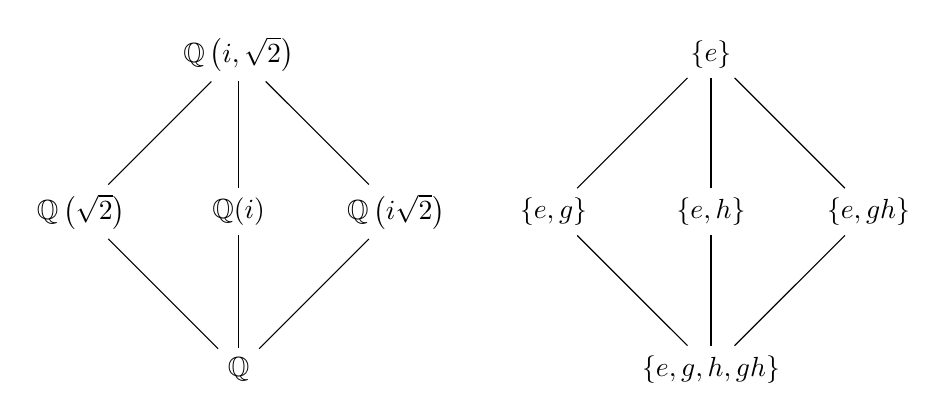
\begin{tikzpicture}[node distance=2cm]
        \node (Q)                  {$\mathbb{Q}$};
        \node (Qi)  [above of=Q]   {$\mathbb{Q}(i)$};
        \node (Qi2) [right of=Qi]  {$\mathbb{Q}\left(i\sqrt{2}\right)$};
        \node (Q2)  [left of=Qi]   {$\mathbb{Q}\left(\sqrt{2}\right)$};
        \node (Q2i) [above of=Qi]  {$\mathbb{Q}\left(i, \sqrt{2}\right)$};
        \node (eg)  [right of=Qi2] {$\{e, g\}$};
        \node (egh) [right of=eg]  {$\{e, h\}$};
        \node (eh)  [right of=egh] {$\{e, gh\}$};
        \node (G)   [below of=egh] {$\{e, g, h, gh\}$};
        \node (e)   [above of=egh] {$\{e\}$};
        \draw (Q)   -- (Qi2);
        \draw (Q)   -- (Q2);
        \draw (Q)   -- (Qi);
        \draw (Qi2) -- (Q2i);
        \draw (Q2)  -- (Q2i);
        \draw (Qi)  -- (Q2i);
        \draw (G)   -- (eg);
        \draw (G)   -- (egh);
        \draw (G)   -- (eh);
        \draw (eg)  -- (e);
        \draw (egh) -- (e);
        \draw (eh)  -- (e);
    \end{tikzpicture}
\end{center}

The recipe for producing an intermediate subfield from a subgroup is to take the elements of $\Q\left(i, \sqrt{2}\right)$ which are fixed by all elements of the subgroup.
For instance, $\Q\left(i \sqrt{2}\right)$ is the field of elements fixed by both $e$ and $gh$.

This correspondence doesn't always work for all finite field extensions.  It works for Galois extensions.
In the correspondence, normal extensions correspond to normal subgroups.
In this example, all subgroups are normal and the extensions are normal.
We'll also prove the Primitive Element Theorem, which in the context of finite extensions of $\Q$ tells us that they are necessarily of the form $\Q(\alpha)$ for some $\alpha$, for instance $\Q(i, \sqrt{2}) = \Q(i + \sqrt{2})$.

\subsection{Review of GRM}
\begin{ndef}[Algebraic]\hypertarget{def:algebraic}
    Suppose $K \leq L$ is a field extension. Take $\alpha \in L$ and define
    \begin{equation*}
        I_\alpha = \set{f \in K[t] | f(\alpha) = 0}
    \end{equation*}
    We say $\alpha$ is \textbf{algebraic} over $K$ if $I_\alpha \ne 0$.  Otherwise $\alpha$ is \textbf{transcendental}.
    We say $L$ is algebraic over $K$ if $\alpha$ is algebraic over $K$ for all $\alpha \in L$.
\end{ndef}

\begin{remark}
    We can see $I_\alpha$ is an ideal of $K[t]$ since it is the kernel of the ring homomorphism $K[t] \to L$ given by $f(t) \mapsto f(\alpha)$.
\end{remark}

\begin{eg}
    \leavevmode
    \begin{enumerate}[label=(\roman*)]
        \item $\sqrt{2}$ is \hyperlink{def:algebraic}{algebraic} over $\Q$
        \item $\pi$ is algebraic over $\Q$
    \end{enumerate}
\end{eg}

\begin{nlemma}\label{lem:1.5}
    Let $K \leq L$ be a \hyperlink{def:degreeOfFieldExt}{finite} \hyperlink{def:fieldExt}{field extension}. Then $L$ is \hyperlink{def:algebraic}{algebraic} over $K$.
\end{nlemma}

\begin{proof}
    Let $\abs{L:K}=n$, and take $\alpha \in L$. Consider $1, \alpha, \alpha^2, \dotsc, \alpha^n$, which must be linearly dependent in the $n$-dimensional $K$--vector space $L$.
    So, $\sum_{i=0}^n \lambda_i \alpha^i = 0$ for some $\lambda \in K$ not all zero, and hence $\alpha$ is a root of $f(t) = \sum_{i=0}^n \lambda_i t^i$, so $\alpha$ is \hyperlink{def:algebraic}{algebraic} over $K$.
    $\alpha$ was arbitrary, so $L$ is algebraic over $K$.
\end{proof}

\begin{ndef}[Minimal polynomial]\hypertarget{def:minimalPoly}
    The non-zero ideal $I_\alpha$ (where $\alpha$ is \hyperlink{def:algebraic}{algebraic} over $K$) is principal since $K[t]$ is a principal ideal domain.
    In particular, we can say $I_\alpha = (f_\alpha(t))$ where $f_\alpha(t)$ can be assumed to be monic.
    Such a monic $f_\alpha(t)$ is the \textbf{minimal polynomial} of $\alpha$ over $K$.
\end{ndef}

\begin{remark}
    Multiplication by $\alpha$ within the field $L$ gives a $K$--linear map $L \to L$, an automorphism (if $\alpha \ne 0$).  In GRM, we have seen the \hyperlink{def:minimalPoly}{minimal polynomial} of a linear map is unique.
\end{remark}

\begin{eg}\leavevmode
    \begin{enumerate}[label=(\roman*)]
        \item The minimal polynomial of $\sqrt{2}$ over $\Q$ is $t^2 - 2$.
        \item The minimal polynomial of $\sqrt{2}$ over $\R$ is $t - \sqrt{2}$.
    \end{enumerate}
\end{eg}

\begin{nlemma}\label{lem:1.7}
    Suppose $K \leq L$ is a \hyperlink{def:fieldExt}{field extension}, $\alpha \in L$ and $\alpha$ is \hyperlink{def:algebraic}{algebraic} over $K$.
    Then the \hyperlink{def:minimalPoly}{minimal polynomial} $f_\alpha(t)$ of $\alpha$ over $K$ is irreducible in $K[t]$ and $I_\alpha$ is a prime ideal.
\end{nlemma}

\begin{proof}
    Suppose $f_\alpha(t) = p(t) q(t)$. We aim to show $p(t)$ or $q(t)$ is a unit in $K[t]$.
    But $0 = f_\alpha(\alpha) = p(\alpha) q(\alpha)$, so $p(\alpha) = 0$ or $q(\alpha) = 0$, without loss of generality take $p(\alpha) = 0$, thus $p(t) \in I_\alpha$.

    But $I_\alpha=(f_\alpha(t))$, so $p(t) = f_\alpha(t) r(t)$, giving $f_\alpha(t) = f_\alpha(t) r(t) q(t)$ and so $r(t) q(t) = 1$ in $K[t]$, and $q(t)$ is a unit, as required.
    Recall from GRM that irreducible elements of $K[t]$ are prime and hence generate prime ideals of $K[t]$. So $I_\alpha$ is a prime ideal.
\end{proof}

\begin{ndef}[Simple extension]\hypertarget{def:genField}
    Suppose $K\leq L$ is a \hyperlink{def:fieldExt}{field extension} and $\alpha \in L$.  $K(\alpha)$ is defined to be the smallest subfield of $L$ containing $K$ and $\alpha$.
    It's called the field \textbf{generated} by $K$ and $\alpha$.  We say that $L$ is a \textbf{simple extension} if $L = K(\beta)$ for some $\beta \in L$.

    Given $\alpha_1, \dotsc, \alpha_n \in L$, $K \leq L$.  $K(\alpha_1, \dotsc \alpha_n)$ is the smallest field containing $\alpha_1, \dotsc, \alpha_n$.
    It is the field generated by $K$ and $\alpha_1, \dotsc, \alpha_n$.

    On the other hand $K[\alpha]$ is the ring generated by $K$ and $\alpha$, in particular the image of $K[t]$ under the map $f(t) \mapsto f(\alpha)$.
\end{ndef}

% new lec (3)

\begin{nthm}\label{thm:1.9}
    Suppose $K \leq L$ is a \hyperlink{def:fieldExt}{field extension} and $\alpha \in L$ is \hyperlink{def:algebraic}{algebraic} over $K$.  Then
    \begin{enumerate}[label=(\roman*)]
        \item  $\hyperlink{def:genField}{K(\alpha)} = K[\alpha]$
        \item $\hyperlink{def:degreeOfFieldExt}{\abs{K(\alpha) : K}} = \deg f_\alpha(t)$ where $f_\alpha(t)$ is the \hyperlink{def:minimalPoly}{minimal polynomial} of $\alpha$ over $K$.
    \end{enumerate}
\end{nthm}

\begin{proof}\leavevmode
    \begin{enumerate}[label=(\roman*)]
        \item Clearly $K[\alpha] \leq K(\alpha)$. We aim to show that any non-zero element $\beta$ of $K[\alpha]$ is a unit, so $K[\alpha]$ is a field.

            By definition of $K[\alpha]$, we have $\beta = g(\alpha)$ for some $g(t) \in K[t]$.
            Since $\beta = g(\alpha) \neq 0$, $g(t) \notin I_\alpha = (f_\alpha(t))$.
            Thus $f_\alpha(t) \nmid g(t)$.

            From \cref{lem:1.7}, $f_\alpha(t)$ is irreducible and $K[t]$ is a PID, we know $\exists r(t), s(t) \in K[t]$ with
            \begin{equation*}r(t) f_\alpha(t) + s(t) g(t) = 1 \in K[t].\end{equation*}
            Hence $s(\alpha) g(\alpha) = 1$ in $K[\alpha]$, and so $\beta = g(\alpha)$ is a unit, as required.
        \item Let $n = \deg f_\alpha(t)$ We'll show that $T = \set{1, \alpha, \alpha^2, \dotsc, \alpha^{n-1}}$ is a $K$--vector space basis of $K[\alpha]$.

            Spanning: If $f_\alpha(t) = t^n + a_{n-1} t^{n-1} + \dots + a_0$ with $a_i \in K$, then $\alpha^n = -a_{n-1} \alpha^{n-1} - \dots - a_0$.
            This implies $\alpha^n$ is a linear combination of $\set{1, \alpha, \alpha^2, \dotsc, \alpha^{n-1}}$, and an easy induction shows that $\alpha^m$ for $m \geq n$ is likewise a linear combination of $\set{1, \alpha, \alpha^2, \dotsc, \alpha^{n-1}}$, so we have spanning.

            Linear independence: Suppose $\lambda_{n-1} \alpha^{n-1} + \dotsc + \lambda_0 = 0$.
            Let $g(t) = \lambda_{n-1} t^{n-1} + \dotsc + \lambda_0$.  Since $g(\alpha) = 0$, we have $g(t) \in I_\alpha = (f_\alpha(t)).$  So $g(t) = 0$ or $f_\alpha(t) \mid g(t)$.
            The latter is not possible since $\deg f_\alpha(t) > \deg g_\alpha(t)$ so $g(t) = 0$ in $K[t]$ and all the $\lambda_i$'s are zero. \qedhere
    \end{enumerate}
\end{proof}

\begin{ncor}\label{cor:1.10}
    If $K \leq L$ is a \hyperlink{def:fieldExt}{field extension} and $\alpha \in L$, then $\alpha$ is \hyperlink{def:algebraic}{algebraic} over $K$ if and only if $K \leq \hyperlink{def:genField}{K(\alpha)}$ is \hyperlink{def:degreeOfFieldExt}{finite}.
\end{ncor}

\begin{proof} \leavevmode
    \begin{itemize}
        \item[($\Rightarrow$)] By \cref{thm:1.9}, $\abs{K(\alpha):K} = \deg \hyperlink{def:minimalPoly}{f_\alpha(t)} \leq \infty$.
        \item [($\Leftarrow$)] \Cref{lem:1.5}
    \end{itemize}
\end{proof}

\begin{ncor}\label{cor:1.11}
    Let $K \leq L$ be a \hyperlink{def:fieldExt}{field extension} with \hyperlink{def:degreeOfFieldExt}{$\abs{L:K} = n$}. Let $\alpha \in L$, then $\deg f_\alpha(t) \mid n$.
\end{ncor}

\begin{proof}
    Use the \nameref{thm:towerLaw} on $K \leq \hyperlink{def:genField}{K(\alpha)} \leq L$.
    We deduce that $\abs{K(\alpha):K}$ divides $\abs{L:K}$.
    \Cref{thm:1.9}(ii) gives $\deg f_\alpha(t) = \abs{K(\alpha) : K}$.
\end{proof}

\subsection{Digression on (Non-)Constructibility}
Schedules mention `other classical problems' and we are now in a position to tackle some of these using \cref{cor:1.11}.

A classical question from Greek geometry concerns the existence or otherwise of constructions using ruler and compasses (where a ruler refers to a single unmarked straight edge).
If you're an expert you can divide a line betwen 2 points into arbitrarily many equal segments, you can bisect an angle, or you can produce parallel lines.
Given a polygon you can produce a square of the same area or double the area. However,
\begin{enumerate}
    \item You cannot duplicate the cube using ruler and compasses (given a cube you can't produce a cube of double the volume)
    \item You cannot trisect the angle $\pi/3$ using ruler and compasses.
    \item The circle cannot be squared using ruler and compasses (given a circle you can't construct a square of the same area)
\end{enumerate}

Assume we're given a set $P_0$ of points in $\R^2$, and we can formalise our operations.
\begin{itemize}[label={}, leftmargin=*]
    \item \textbf{Ruler operation} Draw a straight line through any two points in $P_0$.
    \item \textbf{Compass operation} Draw a circle with the centre being a point in $P_0$ and radius the distance between a pair of points in $P_0$.
\end{itemize}

\begin{ndef}[Constructible]\hypertarget{def:constructible}
    The points of intersection of any two distinct lines or circles drawn using these operations are \textbf{constructible in one step} from $P_0$.
    More generally, a point $\vec{r} \in \R^2$ is \textbf{constructible} from $P_0$ if there is a finite sequence $\vec{r_1}, \vec{r_2}, \dotsc, \vec{r_n} = \vec{r}$ such that $\vec{r_i}$ is constructible in one step from $P_0 \cup \{\vec{r_1}, \dotsc, \vec{r_{i-1}}\}$.
\end{ndef}

\begin{exercise}
    \hyperlink{def:constructible}{Construct} the midpoint of a line between two points.
\end{exercise}

Let $K_0$ be the subfield of $\R$ \hyperlink{def:genField}{generated} by $\Q$ and the co-ordinates of the points in $P_0$.
Let $\vec{r_i} = (x_i, y_i)$ and set $K_i = \hyperlink{def:genField}{K_{i-1} (x_i, y_i)}$.

Thus $K_0 \hyperlink{def:fieldExt}{\leq} K_1 \leq K_2 \leq \dots \leq K_m \leq \R$.

\begin{nlemma}\label{lem:1.13}
    $x_i, y_i$ are both roots in $K_i$ of quadratic polynomials in $K_{i-1}[t]$.
\end{nlemma}

\begin{proof}
    There are three cases for $\vec{r_i}$: line meets line, line meets circle, circle meets circle. We do the second case only here.
    \begin{center}
        \begin{tikzpicture}[scale=1]
            \tkzDefPoint[label=below:$A$](-0.5,1){A}
            \tkzDefPoint[label=below:$B$](3,2){B}
            \tkzDefPoint[label=below:$C$](0,0){C}

            \tkzDrawCircle[R, very thin](C, 2.5cm)
            \tkzDrawSegment[very thin, add=3cm and 1cm](A, B)

            \tkzInterLC[R](A,B)(C,2.5cm) \tkzGetPoints{X}{Y}
            \tkzLabelPoints[above left](X)
            \tkzLabelPoints[above](Y)

            \tkzDrawPoints[fill=black](A,B,C,X,Y)
            % \draw (0, 0) circle [radius=2];
            % \draw (-3, 0) -- (3, 2);
        \end{tikzpicture}
    \end{center}
    The line is defined by two points $A = (p, q)$ and $B = (r, s)$ while the circle is defined with a centre $C = (t, u)$ and radius $w$.
    Then, points $X$ and $Y$ satisfy the equation of the line $\frac{x-p}{r-p} = \frac{y-q}{s-q}$, and the equation of the circle $(x-t)^2 + (y-u)^2 = w^2$.
    Solving these together gives coordinates of $X$ and $Y$ satisfying quadratic polynomials over $K_{i-1}$.
    The other two cases are left as an exercise for the reader.
\end{proof}

% new lec (4)

\begin{nthm}\label{thm:1.14}
    If $\vec{r} = (x, y)$ is \hyperlink{def:constructible}{constructible} from a set $P_0$ of points in $\R^2$ and if $K_0$ is the subfield of $\R$ \hyperlink{def:genField}{generated} by $\Q$ and the coordinates of the points in $P_0$, then the \hyperlink{def:degreeOfFieldExt}{degrees} $\abs{K_0(x) : K_0}$ and $\abs{K_0(y):K_0}$ are powers of two.
\end{nthm}

\begin{proof}
    Continue with the previous notation of $K_i = K_{i-1}(x_i, y_i)$. By the \nameref{thm:towerLaw},
    \begin{equation*}
        \abs{K_i : K_{i-1}} = \abs{K_{i-1} (x, y): K_{i-1}(x)} \abs{K_{i-1}(x) : K_{i-1}}
    \end{equation*}
    But \cref{lem:1.13} tells us that $\abs{K_{i-1}(x):K_{i-1}}$ must be $1$ or $2$ depending on whether the quadratic polynomial arising in the lemma is reducible or not, using \cref{thm:1.9}(ii). Similarly, $\abs{K_{i-1}(x, y):K_{i-1}(x)}$ is 1 or 2.

    So $\abs{K_i: K_{i-1}} = 1, 2 \ \text{or} \ 4$, (but in fact $4$ cannot happen), hence by the \nameref{thm:towerLaw}, $\abs{K_n:K_0} = \abs{K_n:K_{n-1}} \abs{K_{n-1} : K_{n-2}} \dots \abs{K_1:K_0}$ is a power of two.

    If $r = (x, y)$ is constructible from $P_0$, then
    \begin{align*}
        x, y \in K_n \quad \text{and} \quad K_0 &\leq K_0(x) \leq K_n \\
        K_0 &\leq K_0(y) \leq K_n
    \end{align*}
    and the Tower Law again gives that $|K_0(x):K_0|$ and $|K_0(y):K_0|$ are also powers of $2$.
\end{proof}

To use this for proofs about \hyperlink{def:constructible}{non-constructibility} we need to be reasonably expert at working out \hyperlink{def:minimalPoly}{minimal polynomials}.

\begin{nthm}\label{thm:1.15}
    Let $f(t)$ be a primitive integral polynomial.  Then $f(t)$ is irreducible in $\Q[t]$ if and only if it is irreducible in $\Z[t]$.
\end{nthm}

\begin{proof}
    A special case of Gauss' lemma from GRM.
\end{proof}

\begin{nthm}[Eisenstein's criterion]\label{thm:1.16}
    Let $f(t) = a_n t^n + a_{n-1} t^{n-1} + \dots + a_0 \in \Z[t]$.
    Suppose there is a prime $p$ such that
    \begin{enumerate}[label=(\roman*)]
        \item $p \nmid a_n$
        \item $p \mid a_{n-1}, \, p \mid a_{n-2}, \dotsc, p \mid a_0$
        \item $p^2 \nmid a_0$
    \end{enumerate}
    Then $f(t)$ is irreducible in $\Z[t]$
\end{nthm}

\begin{proof}
    Recall from GRM.
\end{proof}

\begin{eg}
    For $p$ a prime, consider $f(t) = t^{p-1} + t^{p-2} + \dots + 1$.  This is irreducible over $\Q$ by considering $f(t+1)$ and using $p$ as the prime in \nameref{thm:1.16}.
\end{eg}

Another method is to consider an integral polynomial $f(t) \pmod{p}$. If $f(t)$ is irreducible in $\Z[t]$ then it is reducible over $\Z / p \Z$. So, if we find a prime $p$ such that $f(t) \pmod{p}$ is irreducible then $f(t)$ is irreducible in $\Z[t]$.

\begin{eg}
    $t^3 + t + 1$ is irreducible mod $2$.
    If it were reducible it would have a linear factor and so the polynomial would have a root mod 2.
    But $0, 1$ are not roots.
    So, $t^3 + t + 1$ is irreducible in $\Z[t]$, hence irreducible in $\Q[t]$.
\end{eg}

\begin{remark}
    On a later example sheet you'll meet an irreducible polynomial in $\Z[t]$ which is reducible mod $p$ for all primes $p$.
\end{remark}

% back to non-constructibility
\begin{nthm}\label{thm:1.17}
    The cube cannot be duplicated by \hyperlink{def:constructible}{ruler and compasses}.
\end{nthm}

\begin{proof}
    The problem amounts to whether given a unit distance, one can construct points distance $\alpha$ apart, where $\alpha$ satisfies $t^3 - 2 = 0$.
    Starting with points $P_0 = \{(0, 0), (1, 0)\}$ can we produce $(\alpha, 0)$?

    No. If we could, \cref{thm:1.14} would say $\abs{\Q(\alpha):\Q}$ is a power of 2. But $\abs{\Q(\alpha): \Q} = 3$ since $\abs{\Q(\alpha):\Q} = \deg f_\alpha(t)$ where $f_\alpha(t)$ is the \hyperlink{def:minimalPoly}{minimal polynomial} of $\alpha$ over $\Q$. $\alpha$ satisfies $t^3 - 2$, which is irreducible over $\Z$ by \nameref{thm:1.16} hence irreducible over $\Q$. So $t^3 - 2$ is the minimal polynomial $f_\alpha(t)$.
\end{proof}

\begin{nthm}\label{thm:1.18}
    The circle cannot be squared using ruler and compasses.
\end{nthm}

\begin{proof}
    Starting with $(0, 0)$ and $(1, 0)$, we must \hyperlink{def:constructible}{construct} $(\sqrt{\pi}, 0)$ so that we have a square of side length $\sqrt{\pi}$ and hence area $\pi$.
    But $\pi$ and hence $\sqrt{\pi}$ is transcendental over $\Q$ (Lindemann - not proved here).
    \Cref{thm:1.14} tells us we can't do this construction.
\end{proof}

\subsection{Return to theory development}
\begin{nlemma}\label{lem:1.19}
    Let $K \leq L$ be a \hyperlink{def:fieldExt}{field extension}. Then
    \begin{enumerate}[label=(\roman*)]
        \item $\alpha_1, \dotsc, \alpha_n \in L$ are \hyperlink{def:algebraic}{algebraic} over $K$ if and only if $K \leq \hyperlink{def:genField}{K(\alpha_1, \dotsc \alpha_n)}$ is a \hyperlink{def:degreeOfFieldExt}{finite} field extension.
        \item If $K \leq M \leq L$ such that $K \leq M$ is \hyperlink{def:degreeOfFieldExt}{finite}, then there exist $\alpha_1, \dotsc \alpha_n \in L$ such that $K(\alpha_1, \dotsc \alpha_n) = M$.
    \end{enumerate}
\end{nlemma}

\begin{proof} \leavevmode
    \begin{enumerate}[label=(\roman*)]
        \item By \cref{cor:1.10}, $\alpha$ is algebraic over $K$ if and only if $K \leq K[\alpha]$ is a \hyperlink{def:degreeOfFieldExt}{finite} field extension.
            $\alpha_i$ is algebraic over $K$ and hence algebraic over $K(\alpha_1, \dotsc \alpha_{i-1})$ and so
            \begin{equation*}\abs{K(\alpha_1, \dotsc, \alpha_i):K(\alpha_1, \dotsc, \alpha_{i-1})} < \infty.\end{equation*}
            By the \nameref{thm:towerLaw} applied to
            \begin{equation*}K \leq K(\alpha_1) \leq K(\alpha_1, \alpha_2) \leq \dots \leq K(\alpha_1, \dotsc \alpha_n),\end{equation*} we get $\abs{K(\alpha_1, \dotsc \alpha_n):K} < \infty$.

            Conversely, consider $K \leq K(\alpha_1) \leq K(\alpha_1, \dotsc \alpha_n)$.
            Then the tower law says that if $\abs{K(\alpha_1, \dotsc, \alpha_n): K} < \infty$ then $\abs{K(\alpha_1):K} < \infty$ and by \cref{cor:1.10}, $\alpha$ is algebraic over $K$.

        \item If $\abs{M:K} = n$ then $M$ is an $n$-dimensional $K$-vector space, so there exists a $K$-basis $\alpha_1, \dotsc, \alpha_n$ over $M$.
            Then $K(\alpha_1, \dotsc, \alpha_n) \leq M$.
            However, any element of $M$ is a $K$-linear combination of $\alpha_1, \dotsc, \alpha_n$ and so lies in $K(\alpha_1, \dotsc, \alpha_n)$, so $M = K(\alpha_1, \dotsc, \alpha_n)$. \qedhere
    \end{enumerate}
\end{proof}

% new lec (5)

\begin{ndef}[Homomorphism over a field]\hypertarget{def:homo}
    Suppose $K \leq L$, $K \leq L'$ are \hyperlink{def:fieldExt}{field extensions}.
    A $K$-\textbf{homomorphism} $\phi: L \to L'$ is a ring homomorphism such that $\phi\vert_K = \id$.

    A $K$-homomorphism is a $K$-isomorphism if it is a ring isomorphism.
\end{ndef}

\begin{nlemma}\label{lem:1.21}
    Suppose $K \leq L$, $K \leq L'$ are \hyperlink{def:fieldExt}{field extensions}. Then
    \begin{enumerate}[label=(\roman*)]
        \item Any \hyperlink{def:homo}{$K$-homomorphism} $\phi:L \to L'$ is injective and $K \leq \phi(L)$ is a field extension.
        \item If $|L:K| = |L':K| < \infty$ then any $K$-homomorphism $\phi:L \to L'$ is a \hyperlink{def:homo}{$K$-isomorphism}.
    \end{enumerate}
\end{nlemma}

\begin{proof} \leavevmode
    \begin{enumerate}[label=(\roman*)]
        \item $L$ is a field and $\ker \phi$ is an ideal of $L$.

            Note $1 \mapsto 1$ and so $\ker \phi$ can't be the whole of $L$, hence $\ker \phi = \{0\}$.
            So $\phi(L)$ is a field and $K \leq \phi(L)$ is a field extension.
        \item $\phi$ is an injective $K$-linear map, so $|\phi(L):K| = |L:K|$.
            In general, $|\phi(L):K| \leq |L':K|$, but since $|L:K| = |L':K|$ by assumption, we have $|\phi(L):K| = |L':K|$, hence $\phi(L) = L'$ and $\phi$ is a $K$-isomorphism $L \to L'$.
            (If $L' = L$ then $\phi$ would be a $K$-automorphism also.) \qedhere
    \end{enumerate}
\end{proof}
% \begin{notation}
%     If $K \leq L$ is a \hyperlink{def:fieldExt}{field extension} and $f(t) \in K[t]$, we denote the set of roots of $f$ in $L$ by $\Root_f(L)$.
% \end{notation}

\begin{ndef}[Splitting]\hypertarget{def:splitting}
    Let $K \leq L$ be a field extension and $f(t) \in K[t]$. We say \textbf{$f$ splits over $L$} if
    \begin{equation*}
        f(t) = a (t-\alpha_1) (t - \alpha_2) \dotsm (t - \alpha_n)
    \end{equation*}
    where $a \in K$ and $\alpha_1, \dotsc, \alpha_n \in L$.

    We say $L$ is a \textbf{splitting field for $f$ over $K$} if $L = K(\alpha_1, \dotsc, \alpha_n)$.
\end{ndef}

\begin{remark}
    This is equivalent to saying that $L$ is a \hyperlink{def:splitting}{splitting field} for $f$ over $K$ iff
    \begin{enumerate}[label=(\roman*)]
        \item $f$ splits over $L$
        \item if $K \leq M \leq L$ and $f$ splits over $M$ then $M=L$.
    \end{enumerate}
\end{remark}

\begin{eg}
    \leavevmode
    \begin{enumerate}
        \item Consider $f(t) = t^3 - 2$ over $\Q$.

            $\Q(\sqrt[3]{2})$ is \emph{not} a \hyperlink{def:splitting}{splitting field} for $f$ over $\Q$, but $\Q(\sqrt[3]{2}, \omega\sqrt[3]{2}, \omega^2\sqrt[3]{2})$ is a splitting field over $\Q$ where $\omega$ is a primitive cube root of unity $\omega = e^{2\pi i/3}$
            \begin{center}
                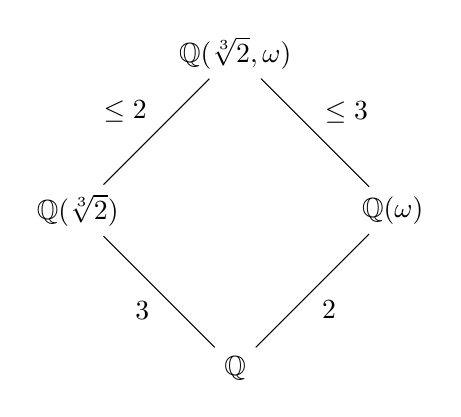
\begin{tikzpicture}[node distance=2cm]
                    \node (blank)                  {};
                    \node (Q2)    [left of=blank]  {$\Q(\sqrt[3]{2})$};
                    \node (Qw)    [right of=blank] {$\Q(\omega)$};
                    \node (Q)     [below of=blank] {$\Q$};
                    \node (Qw2)   [above of=blank]  {$\Q(\sqrt[3]{2}, \omega)$};

                    \draw (Qw2) -- (Qw)  node[midway,anchor=south west]{$\leq 3$}
                                -- (Q)   node[midway,anchor=north west]{$2$}
                                -- (Q2)  node[midway,anchor=north east]{$3$}
                                -- (Qw2) node[midway,anchor=south east]{$\leq 2$};
                \end{tikzpicture}
            \end{center}

            Starting in the bottom right, going clockwise:
            \begin{itemize}
                \item The \hyperlink{def:minimalPoly}{minimal polynomial} of $\omega$ over $\Q$ is $t^2 + t + 1$, so $\hyperlink{def:degreeOfFieldExt}{\abs{\Q(\omega):\Q}}=2$.
                \item $t^3 - 2$ is irreducible over $\Q$ by \nameref{thm:1.16}, so $\abs{\Q(\sqrt[3]{2}):\Q}=3$.
                \item $\omega$ satisfies $t^2 + t + 1$ over $\Q$ and hence over $\Q(\sqrt[3]{2})$ and so $\abs{\Q(\sqrt[3]{2}, \omega):\Q(\sqrt[3]{2})} \leq 2$.
                \item $\sqrt[3]{2}$ satisfies $t^3 - 2$ over $\Q$ and hence over $\Q(\omega)$, so $\abs{\Q(\sqrt[3]{2}, \omega):\Q(\omega)} \leq 3$.
            \end{itemize}

            Then by the \nameref{thm:towerLaw}, $2 \mid \abs{\Q(\sqrt[3]{2}, \omega): \Q}$ and $3 \mid \abs{\Q(\sqrt[3]{2}, \omega): \Q}$, so we deduce
            \begin{align*}
                \abs{\Q(\sqrt[3]{2}, \omega) : \Q(\omega)} = 3 \\
                \abs{\Q(\sqrt[3]{2}, \omega) : \Q(\sqrt[3]{2})} = 2
            \end{align*}

        \item Take $f(t) = (t^2 - 3)(t^3 - 1)$. The splitting field for $f$ over $\Q$ is
            \begin{align*}
                &\Q(\sqrt{3}, -\sqrt{3}, \omega, \omega^2, 1) \\
                = &\Q(\sqrt{3}, \omega) = \Q(\sqrt{3}, i)
            \end{align*}
            since $\omega = \frac{-1 + i \sqrt{3}}{2}$.
        \item $t^2 - 3$ and $t^2 - 2t - 2$ have the same splitting field over $\Q$: $\Q(\sqrt{3})$.
        \item Take $f(t) = t^2 + t + 1$ in $\mathbb{F}_2[t]$.

            $f(t)$ is irreducible over $\mathbb{F}_2$ since it has no roots in $\mathbb{F}_2$ and hence no linear factors in $\mathbb{F}_2[t]$.
            Hence, $\mathbb{F}_2[t]/(t^2 + t + 1)$ is a field.

            Set $\alpha = t + (t^2 + t + 1) \in \mathbb{F}_2[t]/(t^2 + t + 1)$, then
            \begin{equation*}
                \frac{\mathbb{F}_2[t]}{(t^2 + t + 1)} = \mathbb{F}_2[\alpha].
            \end{equation*}

            The elements are $0, 1, \alpha, 1+\alpha$ noting that $\alpha^2 + \alpha + 1 = 0$ and we have characteristic $2$, so $\alpha^2 = \alpha + 1$.

            $f(t)$ splits over $\mathbb{F}_2[\alpha]$:
            \begin{equation*}
                f(t) = (t-\alpha)(t-1-\alpha)
            \end{equation*}
            Thus $\mathbb{F}_2[\alpha]$ is the splitting field for $f$ over $\mathbb{F}_2$.
    \end{enumerate}
\end{eg}
We can use this final construction to produce splitting fields in general.

\begin{nthm}[Existence of splitting fields]\label{thm:1.23}
    Let $K$ be a field and $f(t) \in K[t]$. Then there exists a \hyperlink{def:splitting}{splitting field} for $f$ over $K$.
\end{nthm}

\begin{proof}
    If $\deg f = 0$ then $K$ is the splitting field for $f$ over $K$.

    Suppose $\deg f > 0$ and pick an irreducible factor $g(t)$ of $f(t)$ in $K[t]$, noting that $K \leq K[t] / (g(t))$ is a \hyperlink{def:fieldExt}{field extension}.

    Take
    \begin{equation*}\alpha_1 = t + (g(t)) \in K[t]/(g(t)),\end{equation*}
    then $K[t]/(g(t)) = K(\alpha_1)$ and $g(\alpha_1) = 0$ in $K(\alpha_1)$.
    Therefore $f(\alpha_1) = 0$ in $K(\alpha_1)$ and we can write $f(t) = (t-\alpha_1) h(t)$ in $K(\alpha_1)[t]$.

    Repeat, noting that $\deg h(t) < \deg f(t)$ and so we get
    \begin{equation*}f(t) = a(t - \alpha_1)(t - \alpha_2) \dotsm (t-\alpha_n)\end{equation*}
    where $a$ is a constant in $K$.
    Thus, we have a factorisation of $f(t)$ in $K(\alpha_1, \dotsc, \alpha_n)[t]$, and so $K(\alpha_1, \dotsc, \alpha_n)$ is a splitting field for $f$ over $K$.
\end{proof}

\begin{nthm}[Uniqueness of splitting fields]\label{thm:1.24}
    If $K$ is a field and $f(t) \in K[t]$, then the \hyperlink{def:splitting}{splitting field} for $f$ over $K$ is unique up to \hyperlink{def:homo}{$K$-isomorphism}, that is, if there are two such splitting fields $L$ and $L'$, there is a $K$-isomorphism $\phi: L \to L'$.
\end{nthm}

% new lec (6)

% need to make sure this makes sense
\begin{proof}
    Suppose $L$ and $L'$ are splitting fields for $f(t) \in K[t]$ over $K$. We need to show that there is a $K$-isomorphism $L \to L'$.

    Suppose $K \leq M \leq L$ and there exist $M'$ with $K \leq M' \leq L'$ and a $K$-isomorphism $\psi: M \to M'$.
    Clearly some $M$ exists (we can take $M=K$), so we pick $M$ so that $\abs{M:K}$ is maximal among all such $M, M', \psi$.

    We must show $M=L$ and $M' = L'$. Note that if $M = L$ then $f(t)$ splits over $M$:
    \begin{equation*}
        f(t) = a(t - \alpha_1) \dotsm (t - \alpha_n) \in M[t]
    \end{equation*}
    Apply $\psi$, we get an induced map $M[t] \to M'[t]$.
    \begin{equation*}
        f(t) = \psi(f(t)) = \psi(a) (t - \psi(\alpha_1)) \dotsm (t - \psi(\alpha_n))
    \end{equation*}
    Thus $f(t)$ splits over $\psi(M) = M'$. But $L'$ is a splitting field and $M' \leq L'$, so $M'=L'$.

    So, suppose $M\neq L$ and we'll get a contradiction of maximality of $M$.
    Since $M \neq L$, there is a root $\alpha$ of $f(t)$ in $L$ which isn't in $M$.
    Factorise $f(t) = g(t) h(t)$ in $M[t]$ so that $g(t)$ is irreducible in $M[t]$ while $g(\alpha) = 0$ in $L$.
    Then there exists a $K$-homomorphism $M[t]/(g(t)) \to L$ given by $t + (g(t)) \mapsto \alpha$ which has image $M(\alpha)$.

    The $K$-isomorphism $M[t] \to M'[t]$ induced by $\psi$ maps $g(t) \in M[t]$ to $\gamma(t) \in M'[t]$.
    $f(t) = g(t) h(t)$ in $M[t]$ yields $f(t) = \gamma(t) \delta(t)$ in $M'[t]$.

    We have a field extension $M' \leq M'[t]/(\gamma(t))$ and there exists a $M'$-homomorphism $M'[t]/(\gamma(t)) \to L'$ given by $t + (\gamma(t))$ by picking a root $\alpha'$ of $\gamma(t)$ in $L'$.
    However $\gamma(t) \mid f(t)$ in $M'[t]$ and hence in $L'[t]$ and so $\alpha'$ is also a root of $f(t)$ in $L'$.
    The $M'$-homomorphism gives a $K$-isomorphism
    \begin{equation*}
        M'[t] / (\gamma(t)) \to M'(\alpha')
    \end{equation*}
    and so we have a $K$-isomorphism $M(\alpha) \to M'(\alpha')$. This contradicts the maximality of $M$, since $M \lneqq M(\alpha)$.
\end{proof}

\begin{ndef}[Normal extension]\label{def:1.25}\hypertarget{def:normal}
    A \hyperlink{def:fieldExt}{field extension} $K \leq L$ is \textbf{normal} if for every $\alpha \in L$ the \hyperlink{def:minimalPoly}{minimal polynomial} $f_\alpha(t)$ of $\alpha$ over $K$ \hyperlink{def:splitting}{splits} over $L$.
\end{ndef}

\begin{nthm}\label{thm:1.26}
    Let $K \leq L$ be a \hyperlink{def:degreeOfFieldExt}{finite} \hyperlink{def:fieldExt}{field extension}. Then $K \leq L$ is \hyperlink{def:normal}{normal} $\iff$ $L$ is the \hyperlink{def:splitting}{splitting field} for some $f(t) \in K[t]$.
\end{nthm}

\begin{proof}
    \hyperlink{prf:1.26}{Later.}
\end{proof}

\begin{nexample}\label{thm:1.27}
    Let $\F$ be a finite field with $\abs{\mathbb{F}} = m$. $\F$ has characteristic $p$ for some $p$ and $\F_p \leq \F$, therefore $m = p^r$ for some $r$.
    The non-zero elements form the multiplicative group of order $m-1=n$ and they satisfy $t^n - 1$: they are roots of $t^n - 1$. So,
    \begin{equation*}
        t^n - 1 = (t - \alpha_1) \dotsm (t-\alpha_n)
    \end{equation*}
    where $\alpha_1, \dotsc, \alpha_n$  are the non-zero elements of $\F$. Thus $\F$ is the splitting field for $t^n - 1$ over $\F_p$.
    By \cref{thm:1.24}, any other field with $m$ elements is $\F_p$-isomorphic to $\F$.
    (We'll show later that there is a field of $m$ elements.)
\end{nexample}

\begin{nthm}\label{thm:1.28}
    Let $G$ be a finite subgroup of the multiplicative group of a field $K$. Then $G$ is cyclic. In particular, the multiplicative group of a finite field is cyclic.
\end{nthm}

\begin{proof}
    Let $\abs{G} = n$. By the structure theorem of finite abelian groups from GRM,
    \begin{equation*}
        G \cong C_{q_1^{m_1}} \times C_{q_2^{m_2}} \times \dotsm \times C_{q_r^{m_r}}
    \end{equation*}
    with $q_i$ prime, not necessarily distinct.
    However if $q = q_i = q_j$ for some $i \neq j$, there are at least $q^2$ distinct solutions of $t^q - 1 = 0$ in $K$ (since $C_q \times C_q \cong$ subgroup of $G$).
    But in a field (or even an integral domain), a polynomial of degree $q$ has at most $q$ roots, a contradiction.
    So all the $q_i$ are distinct and hence $G$ is cyclic, generated by $(g_1, \dotsc, g_r)$ where $g_i$ generates $C_{q_i^{m_i}}$ using the Chinese Remainder Theorem.
\end{proof}

\clearpage
\section{Separable, normal and Galois extensions}

\begin{ndef}[Separable polynomial]\hypertarget{def:separablePoly}
    Let $K$ be a field and $f(t) \in K[t]$. Suppose $f(t)$ is irreducible in $K[t]$ and $L$ is a splitting field for $f(t)$ over $K$.
    Then $f(t)$ is \textbf{separable} over $K$ if $f(t)$ has no repeated roots in $L$.

    For general $f(t)$ we say $f(t)$ is separable over $K$ if every irreducible factor in $K[t]$ is separable over $K$.

    All constant polynomials are separable.
\end{ndef}

% new lec (7)

\begin{ndef}[Formal differentiation]\hypertarget{def:diff}
    If $K$ is a field then \textbf{formal differentiation}
    \begin{align*}
        D: K[t] &\to K[t] \\
        t^n &\mapsto n t^{n-1}
    \end{align*}
    is a $K$-linear map.
    We denote this by $D(f(t)) = f'(t)$.
\end{ndef}

\begin{nlemma}\label{lem:2.3}
    Let $K$ be a field and $f(t), g(t) \in K[t]$. Then:
    \begin{enumerate}[label=(\alph*)]
        \item $D(f(t) g(t)) = f'(t) g(t) + f(t) g'(t)$ (Leibniz' rule)
        \item Assume $f(t) \neq 0$. Then $f(t)$ has a repeated root in a splitting field $L$ if and only if $f(t)$ and $f'(t)$ have a common irreducible factor in $K[t]$.
    \end{enumerate}
\end{nlemma}

\begin{proof}
    \leavevmode
    \begin{enumerate}[label=(\alph*)]
        \item \hyperlink{def:diff}{$D$} is a $K$-linear map and so we only need to check for $f(t) = t^n$, $g(t) = t^m$. Left as an exercise.
        \item Let $\alpha$ be a repeated root in a splitting field $L$, then
            \begin{align*}
                f(t) &= (t-\alpha)^2 g(t) \in L[t] \\
                f'(t) &= (t-\alpha)^2 g'(t) + 2(t-\alpha) g(t)
            \end{align*}
            and so $f'(\alpha) = 0$.
            Therefore the \hyperlink{def:minimalPoly}{minimal polynomial} $f_\alpha(t)$ of $\alpha$ in $K[t]$ divides both $f(t)$ and $f'(t)$ and thus $f_\alpha(t)$ is a common irreducible factor of $f(t)$ and $f'(t)$.


            Conversely, let $h(t)$ be a common irreducible factor of $f(t)$ and $f'(t)$ in $K[t]$.
            Pick a root $\alpha$ in $L$ of $h(t)$.

            So $f(\alpha) = 0 = f'(\alpha)$, thus $f(t) = (t-a) g(t)$ in $L[t]$, and $f'(t) = (t-a) g'(t) + g(t)$.
            Since $f'(\alpha)  = 0$ we have $(t-a) \mid f'(t)$. and so $(t-a) \mid g(t)$. Hence $(t-a)^2 \mid f(t)$ and we have a repeated root. \qedhere
    \end{enumerate}
\end{proof}

\begin{ncor}\label{cor:2.4}
    If $K$ is a field and $f(t) \in K[t]$ is irreducible:
    \begin{enumerate}[label=(\roman*)]
        \item If the characteristic of $K$ is 0, then $f(t)$ is \hyperlink{def:separablePoly}{separable} over $K$.
        \item If the characteristic of $K$ is greater than 0, then $f(t)$ is not separable if and only if $f(t) \in K[t^p]$.
    \end{enumerate}
\end{ncor}

\begin{proof}
    By \cref{lem:2.3}, $f(t)$ is not separable over $K$ if and only if $f(t)$ and $f'(t)$ have a common irreducible factor.
    Since we're assuming $f(t)$ is irreducible, this is equivalent to saying $f'(t) = 0$.

    \begin{align*}
        f(t) &= a_n t^n + a_{n-1} t^{n-1} + \dotsb + a_0 \\
        f'(t) &= n a_n t^{n-1} + \dotsb + a_1
    \end{align*}
    Thus $f'(t) = 0 \iff i a_i = 0$ for all $i > 0$.

    \begin{enumerate}[label=(\roman*)]
        \item If $\chara K = 0$ then $f'(t) \neq 0$ for any non-constant polynomial, so $f(t)$ is separable over $K$.
        \item If $\chara K = p > 0$ then if $f'(t) = 0$ we have $i a_i = 0$ for all $i > 0$, so $f(t)$ is not separable $\iff f(t) \in K[t^p]$. \qedhere
    \end{enumerate}
\end{proof}

\begin{ndef}[Separable extension]\hypertarget{def:separableExt}
    We say \textbf{$\alpha \in L$ is separable over $K$} if its \hyperlink{def:minimalPoly}{minimal polynomial} is \hyperlink{def:separablePoly}{separable} over $K$.

    \textbf{$L$ is separable over $K$} if all $\alpha \in L$ are separable over $K$.

    If $\hyperlink{def:minimalPoly}{f_\alpha(t)} = (t-\alpha)^n = t^n - \alpha^n$ where $n$ is a power of $p (=\chara K)$, we say that $\alpha$ is \textbf{purely inseparable over $K$}.
\end{ndef}

\begin{eg}
    \leavevmode
    \begin{enumerate}[label=(\arabic*)]
        \item Let $\Q \subseteq L$ be an \hyperlink{def:algebraic}{algebraic} \hyperlink{def:fieldExt}{field extension}. Then $L$ is \hyperlink{def:separablePoly}{separable} over $\mathbb{Q}$.
        \item Let $L = \F_p(X)$ be the rational functions in $X$ over $\F_p$, and $K = \F_p(X^p)$.
            Then $K \leq L$ is not separable.
            Observe that if $f(t) = t^p - X^p \in K[t]$ then $f'(t) = 0$.
            But $t^p - X^p = (t-X)^p$ in $L[t]$ since the binomial expansion gives other terms divisible by $p$ and hence $0$ since the characteristic is $p$.

            However $f(t)$ is irreducible in $K[t]$:
            Suppose $f(t) = g(t) h(t)$ in $K[t]$ and hence in $L[t]$. So we get $g(t) = (t-X)^r$ for some $0 \leq r < p$ if the factorisation is non-trivial.
            But this would mean $X^r$ was in $K$. However, $\exists$integers $a, b$ such that $ar + bp = 1$.
            So $(X^r)^a (X^p)^b \in K$ and so $X \in K$, thus we'd have $X = \frac{u(X^p)}{v(X^p)}$, a contradiction.

            Thus $f(t) = t^p - X^p$ is the \hyperlink{def:minimalPoly}{minimal polynomial} of $X$ over $K$, thus $X$ is \hyperlink{def:separableExt}{purely inseparable} over $K$ and $K \leq L$ is not separable.
        \item Take $\F$ a finite field with order $m$, a power of $p$ where $\chara \F = p$. Consider $f(t) = t^n - 1$ where $n = m-1$. This is separable over $\F_p$ since we saw that $f(t)$ has distinct linear factors in $\F[t]$.
    \end{enumerate}
\end{eg}

\begin{remark}
    It's useful to have an alternative approach to \hyperlink{def:separableExt}{separability of field extensions} without having to check \hyperlink{def:separablePoly}{separability}
    of \hyperlink{def:minimalPoly}{minimal polynomials} for all elements of the larger field.
    This is where we start thinking about \hyperlink{def:homo}{$K$-homomorphisms}.
\end{remark}

\begin{nlemma}\label{lem:2.6}
    Let $M = \hyperlink{def:genField}{K(\alpha)}$, where $\alpha$ is \hyperlink{def:algebraic}{algebraic} over $K$ and let $f_\alpha(t)$ be the \hyperlink{def:minimalPoly}{minimal polynomial} of $\alpha$ over $K$.

    Then, for any \hyperlink{def:fieldExt}{field extension} $K \leq L$, the number of \hyperlink{def:homo}{$K$-homomorphisms} of $M$ to $L$ is equal to the number of distinct roots of $f_\alpha(t)$ in $L$.
    Thus this number is $\leq \deg f_\alpha(t) = \abs{K(\alpha):K} = \abs{M:K}$.

    \begin{center}
        \begin{tikzpicture}[scale=0.8]
            \node (K) at ( 0,-2)    {$K$};
            \node (L) at ( 2, 2)    {$L$};
            \node (M) at (-2, 0)    {$M = K(\alpha)$};

            \draw (M) -- (K) -- (L);
        \end{tikzpicture}
    \end{center}
\end{nlemma}

\begin{proof}
    We saw in \cref{lem:1.21} that any $K$-homomorphism $M \to L$ is injective, and we have
    \begin{equation*}
        K(\alpha) \cong \frac{K[t]}{(f_\alpha(t))}.
    \end{equation*}
    For any root $\beta$ of $f_\alpha(t)$ in $L$ we can define a $K$-homomorphism
    \begin{align*}
        \frac{K[t]}{(f_\alpha(t))} &\to L \\
        t + (f_\alpha(t)) &\mapsto \beta
    \end{align*}
    Thus we get a $K$-homomorphism $M \to L$.

    Conversely, for any $K$-homomorphism $\phi:M \to L$ the image $\phi(\alpha)$ must satisfy
    \begin{equation*}f_\alpha(\phi(\alpha)) = 0.\end{equation*}
    These processes are inverse to each other, giving a 1-1 correspondence
    \begin{equation*}
        \{K \text{ homomorphisms } M \to L\} \longleftrightarrow \{\text{roots of } f_\alpha(t) \in L\}. \qedhere
    \end{equation*}
\end{proof}

% new lec (8)

\begin{eg}
    Take $K = \Q$, $L = \hyperlink{def:genField}{\Q(\sqrt[3]{2})}$, and use $\alpha = \sqrt[3]{2}$, with \hyperlink{def:minimalPoly}{minimal polynomial} $f_\alpha(t) = t^3 - 2$.

    Then, there is only one \hyperlink{def:homo}{$K$-homomorphism} $M = K(\sqrt[3]{2})  =L \to L$, the identity map.
\end{eg}

\begin{ncor}\label{cor:2.7}
    The number of \hyperlink{def:homo}{$K$-homomorphisms} $\hyperlink{def:genField}{K(\alpha)} \to L = \deg f_\alpha(t) \iff L$ is large enough, in particular $L$ contains a \hyperlink{def:splitting}{splitting field} for $f_\alpha(t)$ and $\alpha$ is \hyperlink{def:separableExt}{separable} over $K$.
\end{ncor}

\begin{proof}
    Immediate from \cref{lem:2.6}.
\end{proof}

\begin{nlemma}\label{lem:2.8}
    Let $K \leq M$ be a \hyperlink{def:fieldExt}{field extension} and $M_1 = \hyperlink{def:genField}{M(\alpha_1)}$ (where $\alpha_1$ is \hyperlink{def:algebraic}{algebraic} over $M$).
    Let $f(t)$ be the \hyperlink{def:minimalPoly}{minimal polynomial} of $\alpha_1$ over $M$ and let $K \leq L$.
    Let $\phi: M \to L$ be a \hyperlink{def:homo}{$K$-homomorphism}. Then there is a correspondence
    \begin{equation*}
        \{\text{Extensions } \phi_1:M_1 \to L \text{ of } \phi\} \longleftrightarrow \{\text{roots of} \ \phi(f(t)) \in L\}.
    \end{equation*}
    \begin{center}
        \begin{tikzpicture}
            \node (K)  at ( 0,-2)    {$K$};
            \node (M)  at (-1, -0.5)    {$M$};
            \node (M1) at (-2, 1)    {$M_1$};
            \node (L)  at ( 2, 2)    {$L$};

            \draw (M1) -- (M) -- (K) -- (L);
        \end{tikzpicture}
    \end{center}
\end{nlemma}

\begin{remark}
    \Cref{lem:2.6} is the special case $M=K$ and $\phi =$ inclusion of $K$ in $L$.
\end{remark}

\begin{proof}
    $f(t)$ is irreducible in $M[t]$, so $\phi(f(t))$ is irreducible in $\phi(M)[t]$.
    Any extension $\phi_1: M \to L$ of $\phi$ produces a root $\phi_1(\alpha_1)$ of $\phi(f(t))$.

    Conversely, given a root $\gamma$ of $\phi(f(t))$ in $L$,
    \begin{equation*}
        M_1 = M(\alpha_1) \cong \frac{M[t]}{(f(t))} \cong \frac{\phi(M)[t]}{(\phi(f(t)))} \cong \phi(M)(\phi) \leq L.
    \end{equation*}
    Thus we get an extension $\phi_1$ of $\phi$ as required.
\end{proof}

\begin{ncor}\label{cor:2.9}
    If $L$ is large enough, the number of $\phi_1$ which extend $\phi$ is equal to the number of distinct roots of $f(t)$ in $L$.
    This is equal to $|M_i:M| \iff \alpha$ is \hyperlink{def:separableExt}{separable} over $M$.
\end{ncor}

\begin{proof}
    Immediate from \cref{lem:2.8}.
\end{proof}

\begin{ncor}\label{cor:2.10}
    Let $K \leq M \leq N$ be finite field extensions, $K \leq L$. Let $\phi: M \to L$ be a $K$-homomorphism.
    Then the number of extensions of $\phi$ to maps $\theta:N \to L$ is $\leq \hyperlink{def:degreeOfFieldExt}{\abs{N:M}}$.
    Moreover, such a $\theta$ exists if $L$ is large enough.
\end{ncor}

\begin{proof}
    Pick $\alpha_1, \dotsc, \alpha_r$ so that $N = \hyperlink{def:genField}{M(\alpha_1, \dotsc, \alpha_r)}$ and set $M_i = M(\alpha_1, \dotsc,\alpha_i)$. Then we've got
    \begin{equation*}
        M \leq M_1 \leq M_2 \leq \dotsb \leq M_r = N.
    \end{equation*}
    Using \cref{lem:2.8}, there are
    \begin{align*}
        \leq& \abs{M_1:M} \text{ extensions } \phi_1 : M_1 \to L \text{ of } \phi \\
        \leq& \abs{M_2:M_1} \text{ extensions } \phi_2 : M_2 \to L \text{ of } \phi \\
        \vdotswithin{\leq}\\
        \leq& \abs{M_r:M_{r-1}} \text{ extensions } \phi_r : M_r \to L \text{ of } \phi
    \end{align*}
    By the \nameref{thm:towerLaw}, the number of extensions $\theta: N \to L$ (recall $N=M_r$) of $\phi:M \to L$ is
    \begin{equation*}
        \leq \abs{M_r:M_{r-1}} \abs{M_{r-1}:M_{r-2}} \cdots \abs{M_1:M} = \abs{N:M}
    \end{equation*}
    where the last part comes from the proof of \cref{lem:2.8} - we need $L$ to contain roots.
\end{proof}

\begin{nremark}\label{rem:2.11}
    This proof together with \cref{cor:2.9} shows that the number of extensions $\theta$ of $\phi$ is equal to $\hyperlink{def:degreeOfFieldExt}{\abs{N:M}}$ iff $L$ is large enough (so that everything splits) and $\alpha_i$ is \hyperlink{def:separableExt}{separable} over \hyperlink{def:genField}{$M(\alpha_1, \dotsc, \alpha_{i-1})$}.
\end{nremark}

\begin{nlemma}\label{lem:2.12}
    Let $K \hyperlink{def:fieldExt}{\leq} N$ be a field extension with $\hyperlink{def:degreeOfFieldExt}{\abs{N:K}} = n$ and $N = \hyperlink{def:genField}{K(\alpha_1, \dotsc, \alpha_r)}$ say.
    Then the following are equivalent:
    \begin{enumerate}[label=(\roman*)]
        \item $N$ is \hyperlink{def:separableExt}{separable} over $K$.
        \item Each $\alpha_i$ is separable over $K(\alpha_1, \dotsc, \alpha_n)$.
        \item If $K \leq L$ is large enough there are exactly $n$ distinct \hyperlink{def:homo}{$K$-homomorphisms} $N \to L$.
    \end{enumerate}
\end{nlemma}

\begin{proof}
    (i) $\Rightarrow$ (ii).
    $N$ is \hyperlink{def:separableExt}{separable} over $K \implies \alpha_i$ is separable over $K$.
    The \hyperlink{def:minimalPoly}{minimal polynomial} of $\alpha_i$ over $K(\alpha_1, \dotsc, \alpha_{i-1})$ divides the minimal polynomial of $\alpha_i$ over $K$ (in $K(\alpha_1, \dotsc, \alpha_{i-1})[t]$).

    So if the latter has distinct roots in a splitting field then the former does.
    So $\alpha_i$ separable over $K \implies \alpha_i$ separable over $K(\alpha_1, \dotsc, \alpha_{i-1})$.

    (ii) $\Rightarrow$ (iii) follows from \cref{rem:2.11}.

    (iii) $\Rightarrow$ (i). Assume (iii) is false and (i) true, aiming for a contradiction.
    So, $\exists \beta \in N$ that is not \hyperlink{def:separableExt}{separable} over $K$, so there are $\lneqq\abs{K(\beta):K}$ $K$-homomorphisms $\phi:K(\beta) \to L$ by \cref{cor:2.7}.

    By \cref{cor:2.10}, $\phi$ extends to $\leq \abs{N:K(\beta)}$ extensions $\theta: N \to L$, and so there are $\lneqq\abs{N:K(\beta)}\abs{K(\beta):K}$ $K$-homomorphisms $N\to L$, contradiction.
\end{proof}

\begin{ndef}[Separably generated]\hypertarget{def:separableGen}
    We say $M = \hyperlink{def:genField}{K(\alpha_1, \dotsc, \alpha_r)}$ is \textbf{separably generated} by $\alpha_1, \dotsc, \alpha_r$ over $K$ if each $\alpha_i$ is \hyperlink{def:separableExt}{separable} over $K$.
\end{ndef}

\begin{ncor}\label{cor:2.14}
    A finite extension is \hyperlink{def:separableExt}{separable} $\iff$ it is \hyperlink{def:separableGen}{separably generated}.
\end{ncor}

\begin{proof}
    \Cref{lem:2.12}.
\end{proof}

\begin{nlemma}\label{lem:2.15}
    If $K \leq M \leq L$ \hyperlink{def:degreeOfFieldExt}{finite} \hyperlink{def:fieldExt}{field extensions}, $M \leq L$, then
    \begin{equation*}
        K \leq M, \; \; M \leq L \text{ are both \hyperlink{def:separableExt}{separable} } \iff K \leq L \text{ is separable}
    \end{equation*}
\end{nlemma}

\begin{proof}
    Example sheet.
\end{proof}

\begin{nexample}
    Take $\F$ a finite field, $\abs{\F} = m$. Multiplicative group of order $n = m - 1$ is cyclic.
    Take a generator $\alpha$, then $\F = \F_p(\alpha)$, and so the \hyperlink{def:minimalPoly}{minimal polynomial} of $\alpha$ divides $t^n - 1$.
    Observe this has distinct roots, which are all of $\F \setminus \{0\}$ since $\alpha^n = 1$.
    So the minimal polynomial of $\alpha$ is \hyperlink{def:separablePoly}{separable}, and $\F = \F_p(\alpha)$ is separable over $\F_p$.
\end{nexample}

% new lec (9)

\begin{nthm}[Primitive Element Theorem]\label{thm:2.17}
    Any \hyperlink{def:degreeOfFieldExt}{finite} \hyperlink{def:separableExt}{separable} extension $K \leq M$ is a \hyperlink{def:genField}{simple} extension, that is, $M = K(\alpha)$ for some $\alpha$, called a primitive element.
\end{nthm}

\begin{proof}
    First deal with the case where $K$ is a finite field. Then $M$ is also finite and we can take $\alpha$ to be a generator of the multiplicative group of $M$, which is cyclic.

    Now assume $K$ is an infinite field.

    Since $K\leq M$ is a finite extension, $M = \hyperlink{def:genField}{K(\alpha_1, \alpha_2, \dotsc, \alpha_n)}$ for some $\alpha_i$.
    It is enough to show that any field $M = K(\alpha, \beta)$ with $\beta$ separable over $K$ is of the form $K(\gamma)$.

    Take $f(t)$ and $g(t)$ to be the \hyperlink{def:minimalPoly}{minimal polynomials} of $\alpha$ and $\beta$ over $K$ and let $L$ be the \hyperlink{def:splitting}{splitting field} for $f(t) g(t)$ over $K(\alpha, \beta)$.
    Say the distinct zeros of $f(t)$ in $L$ are $\alpha = \alpha_1, \dotsc, \alpha_a$ and of $g(t)$ are $\beta = \beta_1, \dotsc, \beta_b$.

    By separability, $b = \deg g(t)$.
    Choose $\lambda \in K$ such that all $\alpha_i + \lambda \beta_j$ are distinct, which is possible since $K$ is infinite.
    Set $\gamma = \alpha + \lambda \beta$.

    Let $F(t) = f(\gamma - \lambda t) \in K(\gamma)[t]$. We have $g(\beta) = 0$ and $F(\beta) = f(\alpha) = 0$. Thus $F(t)$ and $g(t)$ have a common zero.

    Any other common zero would have to be $\beta_j$ for some $j > 1$. But then $F(\beta_j) = f(\alpha + \lambda(\beta - \beta_j))$.
    By assumption, $\alpha + \lambda(\beta - \beta_j)$ is never an $\alpha_i$ and so $F(\beta_j) \neq 0$.
    Separability of $g(t)$ says its linear factors are all distinct, so $(t-\beta)$ is a highest common factor of $F(t)$ and $g(t)$ in $L[t]$.

    However the minimal polynomial $h(t)$ of $\beta$ over $K(\gamma)$ then divides $F(t)$ and $g(t)$ in $K(\gamma)[t]$ and hence in $L[t]$. This implies $h(t) = t - \beta$ and so $\beta \in K(\gamma)$.
    Therefore $\alpha = \gamma - \lambda \beta \in K(\gamma)$ and so $K(\alpha, \beta) \subset K(\gamma)$ and equality holds since $\gamma \in K(\alpha, \beta)$.
\end{proof}

\begin{eg}
    From our example in (link) chapter 1, $\Q \leq \Q(\sqrt{2}, i)$, we had intermediate subfields.
    \begin{center}
        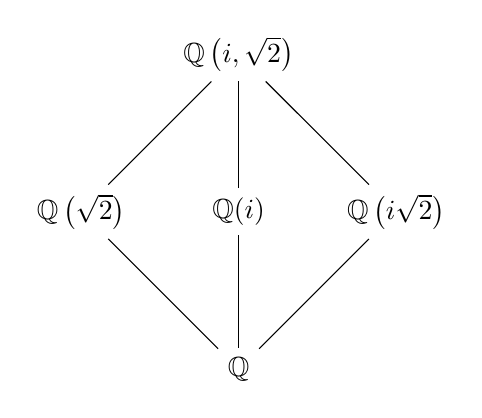
\begin{tikzpicture}[node distance=2cm]
            \node (Q)                  {$\mathbb{Q}$};
            \node (Qi)  [above of=Q]   {$\mathbb{Q}(i)$};
            \node (Qi2) [right of=Qi]  {$\mathbb{Q}\left(i\sqrt{2}\right)$};
            \node (Q2)  [left of=Qi]   {$\mathbb{Q}\left(\sqrt{2}\right)$};
            \node (Q2i) [above of=Qi]  {$\mathbb{Q}\left(i, \sqrt{2}\right)$};
            \draw (Q)   -- (Qi2);
            \draw (Q)   -- (Q2);
            \draw (Q)   -- (Qi);
            \draw (Qi2) -- (Q2i);
            \draw (Q2)  -- (Q2i);
            \draw (Qi)  -- (Q2i);
        \end{tikzpicture}
    \end{center}
    If we follow the procedure of the proof of \cref{thm:2.17}, $\alpha = \sqrt{2}$, $\beta = i$, $f(t) = t^2 - 2$, $g(t) = t^2 + 1$.
    Consider $\sqrt{2} + \lambda i$ where $\pm \sqrt{2} \pm \lambda i$ are distinct.
    For instance $\lambda = 1$, so $\Q(\sqrt{2}, i) = \Q(\sqrt{2}+i)$.
\end{eg}

\subsection{Trace and Norm}

\begin{ndef}[Trace and norm]\hypertarget{def:trNorm}
    Let $K \leq M$ be a \hyperlink{def:degreeOfFieldExt}{finite} \hyperlink{def:fieldExt}{field extension}, and $\alpha \in M$.
    Multiplication by $\alpha$ gives a $K$-linear map $\theta_\alpha: M \to M$.

    Then we define
    \begin{itemize}[label={}]
        \item \textbf{Trace of $\alpha$ over $K$} is given by $\Tr_{M/K}(\alpha) =$ trace of $\theta_\alpha$  $\in K$.
        \item \textbf{Norm of $\alpha$ over $K$} is given by $N_{M/K}(\alpha) =$ determinant of $\theta_\alpha$  $\in K$.
    \end{itemize}

    Note these are dependent on the field extension.
\end{ndef}

\begin{nthm}\label{thm:2.19}
    With the above notation, suppose $f_\alpha(t) = t^s + a_{s-1} t^{s-1} + \dotsb + a_0$ is the \hyperlink{def:minimalPoly}{minimal polynomial} for $\alpha$ over $K$.
    Let $r = \hyperlink{def:degreeOfFieldExt}{\abs{M:K(\alpha)}}$, then the characteristic polynomial of $\theta_\alpha$ is $(f_\alpha(t))^r$.

    Note \begin{equation*}\abs{M:K} = \abs{M:K(\alpha)} |K(\alpha) : K| = rs.\end{equation*}
    Then $\Tr_{M/K} (\alpha) = -r a_{s-1}$ and $N_{M/K} = ((-1)^s a_0)^r$.
\end{nthm}

\begin{proof}
    Regard $M$ as a $K(\alpha)$-vector space with basis $1 = \beta_1, \dotsc, \beta_r$.
    Now take the $K$-vector space basis $1, \alpha, \alpha^2, \dotsc, \alpha^{s-1}$ of $K(\alpha)$.
    So, $1, \alpha, \alpha^2, \dotsc, \alpha^{s-1}, \beta_2, \beta_2 \alpha, \dotsc, \beta_2 \alpha^{s-1}, \beta_3, \dotsc$ is a $K$-vector space basis for $M$.
    Multiplication by $\alpha$ in $K(\alpha)$ is represented by matrix
    \begin{equation*}
        \vec{A} =
        \begin{pmatrix}
            0      & 0      & 0      & \dots  & 0      & -a_0     \\
            1      & 0      & 0      & \dots  & 0      & -a_1     \\
            0      & 1      & 0      & \dots  & 0      & -a_2     \\
            0      & 0      & 1      & \dots  & 0      & -a_3     \\
            \vdots & \vdots & \vdots & \ddots & \vdots & \vdots   \\
            0      & 0      & 0      & \dots  & 1      & -a_{s-1}
        \end{pmatrix}
    \end{equation*}
    an $s \times s$ matrix whose characteristic polynomial is $f_\alpha(t)$.

    Multiplication by $\alpha$ in $M$ is represented by the $rs \times rs$ matrix
    \begin{equation*}
        \begin{pmatrix}
            \vec{A} & 0       & 0       & \dots  & 0       \\
            0       & \vec{A} & 0       & \dots  & 0       \\
            0       & 0       & \vec{A} & \dots  & 0       \\
            \vdots  & \vdots  & \vdots  & \ddots & \vdots  \\
            0       & 0       & 0       & \dots  & \vec{A}
        \end{pmatrix}
    \end{equation*}
    whose characteristic polynomial is $(f_\alpha(t))^r$.

    Look at the terms of this characteristic polynomial to get the trace and norm.
\end{proof}

\begin{nthm}\label{thm:2.20}
    Let $K \leq M$ be a \hyperlink{def:degreeOfFieldExt}{finite} \hyperlink{def:separableExt}{separable} \hyperlink{def:fieldExt}{field extension} and $\hyperlink{def:degreeOfFieldExt}{|M:K| = n}$, $\alpha \in M$.
    Let $K \leq L$ be large enough so that there are $n$ distinct $K$-homomorphisms
    \begin{equation*}
        \sigma_1, \sigma_2, \dotsc, \sigma_n: M \longrightarrow L.
    \end{equation*}
    Then the characteristic polynomial of $\theta_\alpha:M \to M$ (the multiplication map) is
    \begin{equation*}
        \prod_{i=1}^n (t-\sigma_i(\alpha))
    \end{equation*}
    hence
    \begin{equation*}
        \Tr_{M/K} (\alpha) = \sum_{i=1}^n \sigma_i(\alpha) \qquad \text{and} \qquad N_{M/K}(\alpha) = \prod_{i=1}^n \sigma_i(\alpha).
    \end{equation*}
\end{nthm}

\begin{proof}
    Write
    \begin{align*}
        f_\alpha(t) &= (t-\alpha_1) \dotsc (t-\alpha_s) \in L[t] \\
                    &= t^s + a_{s-1} t^{s-1} + \dotsc + a_0
    \end{align*}
    the \hyperlink{def:minimalPoly}{minimal polynomial} of $\alpha$ over $K$ (where $L$ large enough implies $f_\alpha(t)$ splits in $L$).
    There are $s$ \hyperlink{def:homo}{$K$-homomorphisms} $K[\alpha] \to L$ corresponding to maps sending $\alpha$ to $\alpha_i$.

    Each of these extends in $\abs{M:K(\alpha)}$ ways to give $K$-homomorphisms $M \to L$ (by \hyperlink{def:separableExt}{separability} and \cref{cor:2.9}).

    However each of these extensions of a map sending $\alpha \to \alpha_i$ still sends $\alpha \to \alpha_i$.
    Set $r = |L:K(\alpha)|$. Thus there are $r$ maps sending $\alpha \to \alpha_i$ for each $i$.
    Thus if the $n (=rs)$ distinct $K$-homomorphisms $M \to L$ are $\sigma_1, \dotsc, \sigma_n$, then
    \begin{align*}
        \sum_{i=1}^n \sigma_i(\alpha) &= r(\alpha_1 + \alpha_2 + \dotsb + \alpha_s) = -r a_{s-1} = \Tr_{M/K}(\alpha) \\
        \prod_{i=1}^n \sigma_i(\alpha) &= ((-1)^s a_0)^n = N_{M/K}(\alpha). \qedhere
    \end{align*}
\end{proof}

% new lec (10)

\begin{nthm}\label{thm:2.21}
    Let $K \leq M$ be a \hyperlink{def:degreeOfFieldExt}{finite} \hyperlink{def:separableExt}{separable extension}.
    Then we define a $K$-bilinear form
    \begin{align*}
        T: M \times M &\rightarrow K \\
        (x, y) &\longmapsto \Tr_{M/K} (xy).
    \end{align*}
    Then this is non-degenerate and in particular the $K$-linear map $\Tr_{M/K}:M \to K$ is non-zero, and hence surjective.
\end{nthm}

\begin{remark}
    If $K \leq M$ is a finite extension which is not \hyperlink{def:separableExt}{separable} then $\Tr_{M/K}: M \to K$ is always zero and so $T:M\times M \to K$ is degenerate (see example sheet).
\end{remark}

\begin{proof}
    Separability and finiteness give $M=\hyperlink{def:genField}{K(\alpha)}$ for some $\alpha$, by \cref{thm:2.17}.
    We have a $K$-basis $1, \alpha, \alpha^2, \dotsc, \alpha^{n-1}$ of $K(\alpha)$ where $n = \abs{M:K}$.
    The $K$-bilinear form is represented by
    \begin{equation*}
        A =
        \begin{pmatrix}
            \Tr_{M/K}(1)      & \Tr_{M/K}(\alpha)   & \dots  \\
            \Tr_{M/K}(\alpha) & \Tr_{M/K}(\alpha^2) & \dots  \\
            \vdots            & \vdots              & \ddots \\
        \end{pmatrix}.
    \end{equation*}
    Let $L$ be the splitting field of the minimal polynomial $f_\alpha(t)$ of $\alpha$ over $K$.

    Thus $f_\alpha(t) = (t-\alpha_1) \dotsm (t-\alpha_n)$ with $\alpha_1, \dotsc, \alpha_n \in L$.
    The entries in $A$ are of the form $\Tr_{M/K}(\alpha^e)$ which is $\alpha_1^e + \dotsb + \alpha_n^e$ using \cref{thm:2.20}.

    Now consider $\Delta = \prod_{i < j} (\alpha_i - \alpha_j)$, the discriminant of $V$:
    \begin{equation*}
        V =
        \begin{pmatrix}
            1 & 1 & \dots & 1 \\
            a_1 & a_2 & \dots & a_n \\
            a_1^2 & a_2^2 & \dots & a_n^2 \\
            \vdots & \vdots & \ddots & \vdots \\
            a_1^{n-1} & a_2^{n-1} & \dots & a_n^{n-1}
        \end{pmatrix}.
    \end{equation*}
    Observe that $V V^T = A$, and $0 \neq \Delta^2 = \abs{V V^T} = \abs{A}$, so $A$ is non-singular and therefore the bilinear form $T$ is non-degenerate.
\end{proof}

\begin{remark}
    We'll meet $\Delta$ again shortly, as it is the discriminant of the polynomial $f_\alpha(t)$.
\end{remark}

\subsection{Normal extensions}
We restate \cref{def:1.25} and \cref{thm:1.26}:

\begin{manual}{Definition 1.25}[Normal extension]
    An \hyperlink{def:fieldExt}{extension} $K \leq L$ is \textbf{normal} if for every $\alpha \in L$ the \hyperlink{def:minimalPoly}{minimal polynomial} $f_\alpha(t)$ of $\alpha$ over $K$ \hyperlink{def:splitting}{splits} over $L$.
\end{manual}

\begin{manual}{Theorem 1.26}
    Let $K \leq L$ be a \hyperlink{def:degreeOfFieldExt}{finite} \hyperlink{def:fieldExt}{field extension}. Then $K \leq L$ is \hyperlink{def:normal}{normal} $\iff$ $L$ is the \hyperlink{def:splitting}{splitting field} for some $f(t) \in K[t]$.
\end{manual}

\begin{proof}
    \hypertarget{prf:1.26}Assume $K \leq M$ is \hyperlink{def:normal}{normal}. Pick $\alpha_1, \dotsc, \alpha_r \in M$ so that $M = \hyperlink{def:genField}{K(\alpha_1, \dotsc, \alpha_r)}$.
    Let $f_{\alpha_i}(t)$ be the \hyperlink{def:minimalPoly}{minimal polynomial} for $\alpha_i$ over $K$.

    Let \begin{equation*}f(t) = f_{\alpha_1}(t) f_{\alpha_2}(t)  \dotsc f_{\alpha_r}(t).\end{equation*}
    By normality, each $f_{\alpha_i}(t)$ splits over $M$ and therefore $f(t)$ splits over $M$.
    $M$ is the splitting field of $f(t)$ over $K$ since if $\beta_1, \dotsc, \beta_m$ are the roots of $f(t)$ then $M=K(\beta_1, \dotsc, \beta_m)$.

    Conversely, suppose $M$ is a splitting field for $f(t)$ over $K$. Thus $M= K(\beta_1, \dotsc, \beta_m)$ where the $\beta_j$ are the roots of $f(t)$ in $M$.

    Take $\alpha\in M$. Let $f(t)$ be the minimal polynomial of $\alpha$ over $K$.
    Let $M \leq L$ large enough so that $f_\alpha(t)$ splits in $L$ and consider \hyperlink{def:homo}{$K$-homomorphisms} $\phi:M \to L$.
    $\phi(\beta_j)$ is also a root of $f(t)$ and is therefore one of the $\beta_j$s.
    Injectivity of $K$-homomorphisms (\cref{lem:1.21}) implies that $\phi$ generate the $\beta_j$.

    $M = K(\beta_1, \dotsc, \beta_m)$ and so $\phi$ is determined by the images of the $\beta_j$ and thus $\phi(M) = M$.
    However if $\alpha_i$ is a root of $f_\alpha(t)$ in $L$, there is a $K$-homomorphism
    \begin{align*}
        K(\alpha) &\longrightarrow K(\alpha_i) \leq L \\
        \alpha &\longmapsto \alpha_i.
    \end{align*}
    This extends by \cref{cor:2.10} to a \hyperlink{def:homo}{$K$-homomorphism} $\phi: M \to L$ with $\phi(\alpha) = \alpha_i$.
    But $\phi(M) = M$, so $\alpha_i \in M$. Thus $M$ is normal over $K$.
\end{proof}

\begin{remark}
    As for \hyperlink{def:separableExt}{separability}, the property of `\hyperlink{def:normal}{normality}' is equivalent to `normally generated'.
    In particular, a \hyperlink{def:degreeOfFieldExt}{finite extension} $K \leq L$ is normal if and only if $L = \hyperlink{def:genField}{K(\alpha_1, \dotsc, \alpha_r)}$, with each $\hyperlink{def:minimalPoly}{f_{\alpha_i}}(t)$ \hyperlink{def:splitting}{splitting} over $L$.
\end{remark}

\begin{ndef}[Automorphism group]\hypertarget{def:autGroup}
    Let $K \leq M$ be a \hyperlink{def:degreeOfFieldExt}{finite} \hyperlink{def:fieldExt}{field extension}.
    Its \textbf{$K$-automorphism} group is $\Aut_K(M) = \set{\phi | \phi \text{ a \hyperlink{def:homo}{$K$-homomorphism} } M \to M}$.
\end{ndef}

From \cref{lem:1.21} we know that such \hyperlink{def:homo}{$K$-homomorphisms} are isomorphisms and thus have inverses. Composition gives the group operation.

\begin{nlemma}\label{lem:2.23}
    \begin{equation*}
        \Aut_K(M) \leq \abs{M:K}.
    \end{equation*}
\end{nlemma}

\begin{proof}
    \Cref{cor:2.10}.
\end{proof}

\begin{nthm}\label{thm:2.24}
    Let $K \leq M$ be a \hyperlink{def:degreeOfFieldExt}{finite} \hyperlink{def:fieldExt}{field extension}.
    Then $\abs{\hyperlink{def:autGroup}{\Aut_K}(M)} = \hyperlink{def:degreeOfFieldExt}{\abs{M:K}}$ iff the extension is both \hyperlink{def:normal}{normal} and \hyperlink{def:separableExt}{separable}.
\end{nthm}

\begin{ndef}[Galois extension]\hypertarget{def:galoisExt}
    A \hyperlink{def:degreeOfFieldExt}{finite} \hyperlink{def:fieldExt}{field extension} that is \hyperlink{def:normal}{normal} and \hyperlink{def:separableExt}{separable} is a \textbf{Galois extension}.
\end{ndef}

% new lec (11)

\begin{ndef}[Galois group]\hypertarget{def:galoisGroup}
    Let $K \leq M$ be a \hyperlink{def:galoisExt}{Galois extension}.
    Then, the $K$-\hyperlink{def:autGroup}{automorphism group} of $M$ is the \textbf{Galois group} of $M$ over $K$.
    Write this as $\Gal(M / K)$.
\end{ndef}

\begin{remark}
    Some authors use `Galois group' for the \hyperlink{def:autGroup}{automorphism group} even when the extension is not \hyperlink{def:galoisExt}{Galois}.
\end{remark}

% check this makes sense
\begin{proof}[Proof of \cref{thm:2.24}]
    $(\Rightarrow$). Suppose $\abs{\hyperlink{def:autGroup}{\Aut_K}(M)} = \hyperlink{def:degreeOfFieldExt}{\abs{M:K}} = n$.
    Let $L$ be large enough containing $M$.

    The $n$ distinct \hyperlink{def:homo}{$K$-homomorphisms} $\phi: M \to M \leq L$ give us $n$ $K$-homomorphisms $\phi:M \to L$ and \cref{lem:2.12} says that $M$ is separable over $K$.
    For normality, pick $\alpha \in M$ with \hyperlink{def:minimalPoly}{minimal polynomial} $f_\alpha(t)$ over $K$.

    Take $M = K(\alpha_1, \dotsc, \alpha_m)$ as in the proof of \cref{cor:2.10} with $\alpha = \alpha_1$ and $L = M$.
    We only get $\abs{M:K}$ extensions of the inclusion $K \hookrightarrow M$ if each inequality in the proof is an equality.
    In particular we need the number of $K$-homomorphisms $K(\alpha_1) \to M$ to be $\abs{K(\alpha_1):K}$.

    But then \cref{lem:2.6} says we have $\abs{K(\alpha):K}$ distinct roots of $f_\alpha(t)$ in $M$.
    Thus $f_\alpha(t)$ \hyperlink{def:splitting}{splits} over $M$.

    Conversely, suppose $K \leq M$ is separable and normal.
    Then for $K \leq M \leq L$ with $L$ large enough, separability implies there are $\abs{M:K}$ \hyperlink{def:homo}{$K$-homomorphisms} $\phi:M \to L$ by \cref{lem:2.12}.
    However since $K \leq M$ is normal, it is the splitting field for some polynomial $f(t) \in K[t]$ (\cref{thm:1.26}) and thus $M = K(\alpha_1, \dotsc, \alpha_n)$, where $f(t) = (t - \alpha_1) \dotsm (t - \alpha_n)$.
    Note that $\phi(a_j)$ is also a root of $\phi(f(t)) = f(t)$ and is therefore one of the $\alpha_j$s.
    Thus $\phi(M) = M$. Thus we have $\abs{M:K}$ $K$-homomorphisms $\phi:M \to M$.
\end{proof}

\begin{nremark}\label{rem:2.27}
    In the proof we have shown that if $K \leq M \leq L$ and $\phi:M \to L$ is a \hyperlink{def:homo}{$K$-homomorphism} and $K \leq M$ is \hyperlink{def:normal}{normal}, then $\phi(M) = M$.
\end{nremark}

\begin{eg}\leavevmode
    \begin{enumerate}[label=(\arabic*)]
        \item $\Q \leq \Q(\sqrt{2}, i)$ is \hyperlink{def:galoisExt}{Galois}. $\hyperlink{def:galoisGroup}{\Gal}(\Q(\sqrt{2}, i)/\Q)$ has 4 elements:
            \begin{align*}
                \sigma: \sqrt{2} &\longmapsto \pm \sqrt{2} \\
                               i &\longmapsto \pm i
            \end{align*}
            In particular, $\Gal(\Q(\sqrt{2}, i)/\Q) \cong C_2 \times C_2$, all non-identity elements have order 2.
        \item Consider $f(t) = t^3 - 2$. The \hyperlink{def:splitting}{splitting field} over $\Q$ is $\Q(\sqrt[3]{2}, \omega)$, where $\omega$ is a primitive cube root of 1.

            Thus $\Q \leq \Q(\sqrt[3]{2}, \omega)$ is Galois and $\abs{\Q(\sqrt[3]{2}, \omega):\Q} = 6$ (we saw this in the example before \cref{thm:1.23}).
            \begin{align*}
                \sigma_1&:
                    \begin{cases}
                        \sqrt[3]{2} &\longmapsto \sqrt[3]{2} \\ \omega &\longmapsto \omega
                    \end{cases}
                    &&\text{identity} \\
                \sigma_2&:
                    \begin{cases}
                        \sqrt[3]{2} &\longmapsto \omega\sqrt[3]{2} \\ \omega &\longmapsto \omega
                    \end{cases}
                    &&\text{order } 3 \\
                \sigma_3&:
                    \begin{cases}
                        \sqrt[3]{2} &\longmapsto \omega^2\sqrt[3]{2} \\ \omega &\longmapsto \omega
                    \end{cases}
                    &&\text{order } 3 \\
                \sigma_4&:
                    \begin{cases}
                        \sqrt[3]{2} &\longmapsto \sqrt[3]{2} \\ \omega &\longmapsto \omega^2
                    \end{cases}
                    &&\parbox{15em}{complex conjugation\\ order $2$} \\
                \sigma_5&:
                    \begin{cases}
                        \sqrt[3]{2} &\longmapsto \omega^2\sqrt[3]{2} \\ \omega &\longmapsto \omega^2
                    \end{cases}
                    &&\text{order } 2 \\
                \sigma_6&:
                    \begin{cases}
                        \sqrt[3]{2} &\longmapsto \omega\sqrt[3]{2} \\ \omega &\longmapsto \omega^2
                    \end{cases}
                    &&\text{order } 2
            \end{align*}
            Observe also $\sigma_4 \sigma_2 \sigma_4^{-1} = \sigma_3$, so this is the dihedral group.
    \end{enumerate}
\end{eg}

\clearpage
\section{Fundamental Theorem of Galois Theory}
\subsection{Artin's Theorem}
\begin{ndef}[Fixed field]\hypertarget{def:fixedField}
    Let $K \leq L$ be a \hyperlink{def:fieldExt}{field extension} and $H \leq \hyperlink{def:autGroup}{\Aut_K}(L)$.
    The \textbf{fixed field} of $H$ is,
    \begin{equation*}
        L^H \coloneqq \set{\alpha \in L | \sigma(\alpha) = \alpha \text{ for all } \sigma \in H}
    \end{equation*}
\end{ndef}

\begin{ex}
    Check it is a field and $K \leq \hyperlink{def:fixedField}{L^H} \leq L$.
\end{ex}

\begin{nthm}[Fundamental Theorem of Galois Theory]\label{thm:3.2}
    Let $K \leq L$ be a \hyperlink{def:degreeOfFieldExt}{finite} \hyperlink{def:galoisExt}{Galois extension}.
    Then
    \begin{enumerate}[label=(\roman*)]
        \item there is a $1$ to $1$ correspondence
            \begin{align*}
                \{\text{intermediate subfields }K \leq M \leq L\} &\longleftrightarrow \{\text{subgroups $H$ of } \hyperlink{def:galoisGroup}{\Gal}(L/K)\} \\
                M &\longmapsto \hyperlink{def:autGroup}{\Aut_M}(L) \\
                \hyperlink{def:fixedField}{L^H} &\longmapsfrom H
            \end{align*}
            This is called the Galois correspondence.
        \item $H$ is a normal subgroup of $\Gal(L/K)$ iff $K \leq L^H$ is \hyperlink{def:normal}{normal} iff $K \leq L^H$ is \hyperlink{def:galoisExt}{Galois}.
        \item If $H \lhd \Gal(L/K)$ then the map
            \begin{equation*}
                \theta: \Gal(L/K) \longrightarrow \Gal(L^H/K)
            \end{equation*}
            given by restriction to $L^H$ is a surjective group homomorphism with kernel $H$.
    \end{enumerate}
\end{nthm}

\begin{remark}\leavevmode
    \begin{enumerate}[label=(\roman*)]
        \item Observe that $M \leq L$ is \hyperlink{def:galoisExt}{Galois} and so we could have written $\hyperlink{def:galoisGroup}{\Gal}(L/M)$ instead of $\hyperlink{def:autGroup}{\Aut_M}(L)$ in (i).
            To see this: \hyperlink{def:separableExt}{separability} follows from \cref{lem:2.15}.
            \hyperlink{def:normal}{Normality}: If $\alpha \in L$, the \hyperlink{def:minimalPoly}{minimal polynomial} of $\alpha$ over $M$ divides the minimal polynomial of $\alpha$ over $K$.
            But the latter splits over $L$.
        \item If $K \leq M$ is normal then \cref{rem:2.27} says that if $\sigma: L \to L$ then $\sigma(M) = M$ and so we can talk about the restriction of $\alpha$ to $M$ giving an \hyperlink{def:homo}{automorphism} of $M$.
    \end{enumerate}
\end{remark}

\begin{eg} \leavevmode
    \begin{enumerate}[label=(\roman*)]
        \item $\mathbb{Q} \leq \mathbb{Q}(\sqrt{2}, i)$. We saw in \cref{sec:1} the lattice of intermediate fields and subgroups $\Gal(\Q(\sqrt{2}, i)/\Q) \cong C_2 \times C_2$ abelian.
            All subgroups are normal and intermediate subfields are \hyperlink{def:normal}{normal} extensions of $\Q$.
        \item $\Q \leq \Q(\sqrt[3]{2}, \omega)$:
            \begin{center}
                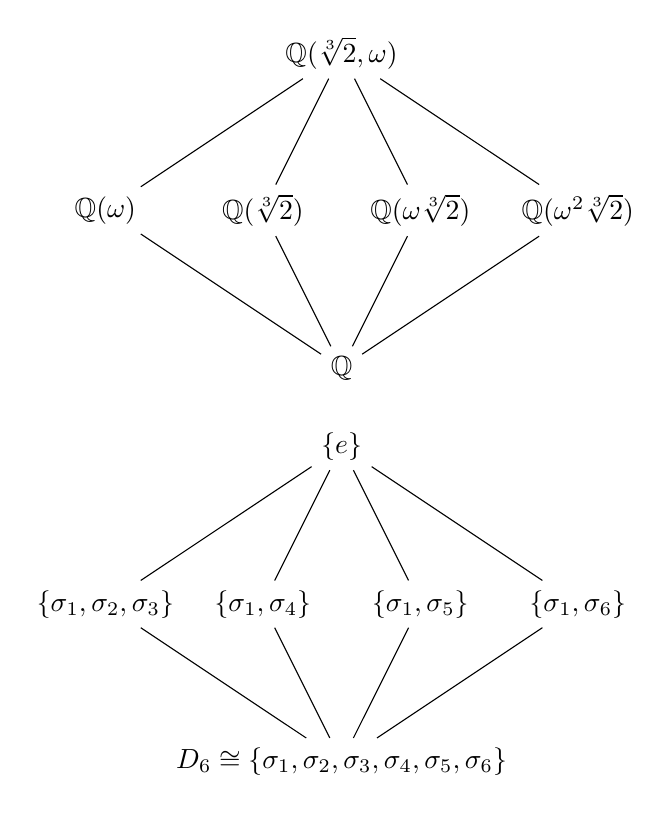
\begin{tikzpicture}
                    \node (Q2-w)   at ( 0, 2)    {$\Q(\sqrt[3]{2}, \omega)$};
                    \node (Qw)     at (-3, 0)    {$\Q(\omega)$};
                    \node (Q2)     at (-1, 0)    {$\Q(\sqrt[3]{2})$};
                    \node (Qw-2)   at ( 1, 0)    {$\Q(\omega \sqrt[3]{2})$};
                    \node (Qw2-2)  at ( 3, 0)    {$\Q(\omega^2 \sqrt[3]{2})$};
                    \node (Q)      at ( 0,-2)    {$\Q$};

                    \foreach \x in {(Qw), (Q2), (Qw-2), (Qw2-2)}{
                        \draw (Q2-w) -- \x -- (Q);
                        };
                    \begin{scope}[yshift=-5cm]
                        \node (Q2-w)   at ( 0, 2)    {$\{e\}$};
                        \node (Qw)     at (-3, 0)    {$\{\sigma_1, \sigma_2, \sigma_3\}$};
                        \node (Q2)     at (-1, 0)    {$\{\sigma_1, \sigma_4\}$};
                        \node (Qw-2)   at ( 1, 0)    {$\{\sigma_1, \sigma_5\}$};
                        \node (Qw2-2)  at ( 3, 0)    {$\{\sigma_1, \sigma_6\}$};
                        \node (Q)      at ( 0,-2)    {$D_6 \cong \{\sigma_1, \sigma_2, \sigma_3, \sigma_4, \sigma_5, \sigma_6\}$};

                        \foreach \x in {(Qw), (Q2), (Qw-2), (Qw2-2)}{
                            \draw (Q2-w) -- \x -- (Q);
                            };
                    \end{scope}
                \end{tikzpicture}
            \end{center}
            The subgroup $H$ of order 3 is normal but those of order 2 are not.
            \begin{equation*}
                \Q \leq \Q(\omega) \text{ is normal} \longleftrightarrow H \text{ of order } 3
            \end{equation*}
            \begin{align*}
                \Gal(\Q(\sqrt[3]{2}, \omega)/\Q) &\longmapsto \Gal(\Q(\omega)/\Q) \\
                D_6 &\longmapsto C_2
            \end{align*}
            This final mapping has kernel $H$, and the image is generated by conjugation.
    \end{enumerate}
\end{eg}

% new lec (12)

\begin{nthm}[Artin's Theorem]\label{thm:3.3}
    Let $K \leq L$ be a \hyperlink{def:fieldExt}{field extension} and $H$ a finite subgroup of $\hyperlink{def:autGroup}{\Aut_K}(L)$.
    Let $M = \hyperlink{def:fixedField}{L^H}$.
    Then $M \leq L$ is a \hyperlink{def:degreeOfFieldExt}{finite} \hyperlink{def:galoisExt}{Galois} extension, and $H = \hyperlink{def:galoisGroup}{\Gal}(L/M)$.
\end{nthm}

\begin{remark}
    This implies some of the Galois correspondence
    \begin{equation*}
        \begin{tikzcd}
            H \arrow[r] & L^H \arrow[r] & \Gal(L / L^H)
        \end{tikzcd}
    \end{equation*}
    we get back to $H$.
\end{remark}

\begin{proof}[Proof of \nameref{thm:3.3}]
    Take $\alpha \in L$. \\
    \textbf{First step:} Show that $\abs{M(\alpha):M} \leq \abs{H}$.
    Let \begin{equation*}\underbrace{\{\alpha_1, \dotsc, \alpha_n\}}_{\text{all distinct}} = \set{\phi(\alpha) | \phi \in H}.\end{equation*}

    Define $g(t) = \prod_{i=1}^n (t-\alpha_i)$.
    Each $\phi$ induces a homomorphism $L[t] \to L[t]$ that sends $g(t)$ to itself, since $\phi$ is permuting the $\alpha_i$.
    So the coefficients of $g(t)$ are fixed by all $\phi \in H$ and thus they all lie in $L^H = M$.
    Thus $g(t) \in M[t]$.

    By definition, $g(\alpha) = 0$ since $\alpha$ is one of the $\alpha_i$.
    Hence the minimal polynomial $f_\alpha(t)$ of $\alpha$ over $M$ divides $g(t)$.
    Thus $\abs{M(\alpha):M} = \deg f_\alpha(t) \leq \deg g(t) \leq \abs{H}$.
    We've shown that $\alpha$ is algebraic over $M$.
    Moreover, $f_\alpha(t)$ is separable since $g(t)$ is.
    Thus $M \leq L$ is a separable extension.

    \textbf{Next step:} Show that $M \leq L$ is a simple extension.
    Pick $\alpha \in L$ with $\abs{M(\alpha):M}$ maximal.
    We'll show that $L = M(\alpha)$ for this choice of $\alpha$.
    Suppose $\beta \in L$. Then $M \leq M(\alpha, \beta)$ is finite and is \hyperlink{def:separableGen}{separably generated} and hence is a finite separable extension by \cref{lem:2.12}.

    By the \nameref{thm:2.17}, $M(\alpha, \beta) = M(\gamma)$ for some $\gamma$.
    But $M \leq M(\alpha) \leq M(\gamma)$.
    The maximality of $\abs{M(\alpha):M}$ forces $M(\alpha) = M(\gamma)$.
    Thus $\beta \in M(\gamma) = M(\alpha)$ and so $L = M(\alpha)$ so $\abs{L:M} \leq \abs{H}$.

    \textbf{Finally,}
    \begin{equation*}
        \abs{L:M} = \abs{M(\alpha):M} \leq \abs{H} \leq \abs{\Aut_M(L)} \underset{\mathclap{
        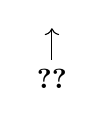
\begin{tikzpicture}
            \node[below] (A) at (0,0) {\Cref{lem:2.23}};
            \draw[->] (A) to (0, 0.4);
        \end{tikzpicture}
        }}{\leq} \abs{L:M}
    \end{equation*}
    We must have equality throughout, and so $\abs{L:M} = \abs{\Aut_M(L)} = \abs{H}$.
    Hence by \cref{thm:2.24} we have $M \leq L$ is a finite Galois extension and $H = \Gal(L/M)$.
\end{proof}

\begin{nthm}\label{thm:3.4}
    Let $K \leq L$ be a \hyperlink{def:degreeOfFieldExt}{finite} \hyperlink{def:fieldExt}{field extension}. Then the following are equivalent:
    \begin{enumerate}[label=(\roman*)]
        \item $K \leq L$ is \hyperlink{def:galoisExt}{Galois}
        \item $\hyperlink{def:fixedField}{L^H} = K$ when $H = \hyperlink{def:autGroup}{\Aut_K}(L)$
    \end{enumerate}
\end{nthm}

\begin{remark}
    The theorem allows some authors yet another alternative definition of a `Galois extension'.
\end{remark}

\begin{proof}
    \textbf{(i) $\Rightarrow$ (ii):} Let $M = L^H$ where $H = \Aut_K(L)$.
    By \nameref{thm:3.3}, $M \leq L$ is a Galois extension, and $\abs{L:M} = \abs{\Gal(L/M)}$ and $H = \Gal(L/M)$.

    However if $K \leq L$ is Galois then $\abs{H} = \abs{\Aut_K(L)} = \abs{L:K}$ by \cref{thm:2.24}.
    Thus $\abs{L:M} = \abs{L:K}$ and so $M = K$.

    \textbf{(ii) $\Leftarrow$ (i):} Use \cref{thm:3.3}.
\end{proof}

\begin{proof}[Proof of \nameref{thm:3.2}]
    \leavevmode
    \begin{enumerate}[label=(\roman*)]
        \item Composing the maps $H \to L^H$ and $M \to \hyperlink{def:galoisGroup}{\Gal}(L /M)$ gives $H \to H$ by \cref{thm:3.3}.
            Also $M \longrightarrow \Gal(L/M) \longrightarrow L^H$ where $H = \Gal(L/M)$ yields $M$ since $M \leq L^H$ where $H = \Gal(L/M)$ and
            \begin{equation*}
                \abs{L:L^H} \underset{\begin{subarray}{c}(\ref{thm:2.24})\\(\ref{thm:3.3})\end{subarray}}{=} \abs{H} = \abs{\Gal(L/M)} \underset{(\ref{thm:2.24})}{=} \abs{L:M}
            \end{equation*}
            So $M = L^H$.
        \item Take $H \leq \Gal(L/K)$, then $L^{\phi H \phi^{-1}} = \phi(L^H)$ when $\phi \in \Gal(L/K)$.
            So by (i), $H$ is \hyperlink{def:normal}{normal} iff $\phi(L^H) = L^H$. Set $M = L^H$.

            We'll show that $K \leq M$ is normal iff $\phi(M) = M \quad \forall \phi \in \Gal(L/K)$.
            $K \leq M$ is normal $\implies \phi(M) = M$ by remark 2 after the statement of \nameref{thm:3.2}.

            Conversely if $\phi(M) = M \quad \forall \phi \in \Gal(L/K)$, pick $\alpha \in M$ and let $f_\alpha(t)$ be its minimal polynomial over $K$.
            Take $\beta$ to be a root of $f_\alpha(t)$ in $L$ (possible by normality).
            Then there is a $K$-homomorphism
            \begin{equation*}
                \begin{tikzcd}[row sep=tiny, column sep=small]
                    K(\alpha) \cong \frac{K[t]}{(f_\alpha(t))} \ar[r] & K(\beta) \cong \frac{K[t]}{(f_\alpha(t))} \leq L \\
                    \alpha \ar[r, mapsto] & \beta.
                \end{tikzcd}
            \end{equation*}
            This extends to a $K$-homomorphism $\phi:L \to L$.

            However we are assuming $\phi(M) = M$ and so $\phi(\alpha) = \beta \in M$. Thus $K \leq M$ is normal.
            Note that $K \leq L^H$ is \hyperlink{def:separableExt}{separable} since $K \leq L^H \leq L$ and $K \leq L$ separable.

        \item By remark 2 after statement of \cref{thm:3.2}, the restriction map
            \begin{equation*}\theta:\Gal(L/K) \rightarrow \Gal(L^H/K)\end{equation*}
            is defined.
            Surjectivity follows from being able to extend a $K$-homomorphism $L^H \to L^H \leq L$ to a $K$-homomorphism $L \to L$ by \cref{cor:2.10}.
            Clearly $H \leq \Ker \theta$. However
            \begin{align*}
                \frac{\abs{L:K}}{\abs{\Ker \theta}} &= \frac{\Gal(L/K)}{\abs{\Ker \theta}} \\
                                                    &= \abs{\Gal(L^H/K)} \quad \text{by surjectivity of } \theta \\
                                                    &= \abs{L^H:K} \quad \text{since } K \leq L^H \text{ is Galois} \\
                                                    &= \frac{\abs{L:K}}{\abs{L:L^H}} \quad \text{by Tower law}
            \end{align*}
            So $\abs{\Ker \theta} = \abs{L:L^H} = \abs{\Gal(L/L^H)} = \abs{H}$ by \cref{thm:3.3}, so $H = \Ker \theta$. \qedhere
    \end{enumerate}
\end{proof}

\subsection{Galois groups of polynomials}
\begin{ndef}[Galois group of polynomial]\hypertarget{def:ggPoly}
    Let $f(t)$ be a \hyperlink{def:separablePoly}{separable} polynomial $\in K[t]$ and let $K \hyperlink{def:fieldExt}{\leq} L$ with $L$ a \hyperlink{def:splitting}{splitting field} for $f(t)$.
    Then the \textbf{Galois group of $f(t)$} over $K$ is
    \begin{equation*}
        \Gal(f) \coloneqq \hyperlink{def:galoisGroup}{\Gal}(L/K).
    \end{equation*}
\end{ndef}

Since $L$ is a splitting field for $f(t)$, $L = \hyperlink{def:genField}{K(\alpha_1, \dotsc, \alpha_n)}$ where $\alpha_1, \dotsc, \alpha_n$ are the roots of $f(t)$ in $L$.
Observe that if $\phi \in \Gal(L/K)$ it maps
\begin{equation*}
    \{\text{roots of } f(t)\} \longrightarrow \{\text{roots of } f(t)\}
\end{equation*}
Thus $\phi$ permutes the $\alpha_i$.
Moreover, if $\phi$ fixes each $\alpha_i$, it also fixes all elements of $L$, and so is the identity map.
Thus $\Gal(f)$ may be regarded as a permutation group of the $n$ roots, so $\Gal(f) \leq S_n$.

\begin{nlemma}\label{lem:3.6}
    Suppose $f(t)$ is \hyperlink{def:separablePoly}{separable}, $f(t) = g_1(t) \dotsm g_s(t)$ with $g_i(t)$ irreducible in $K[t]$ is a factorisation in $K[t]$.
    Then the orbits of $\hyperlink{def:ggPoly}{\Gal}(f)$ on the roots of $f(t)$ correspond to the factors $g_j(t)$.
    \begin{equation*}
        \text{Two roots are in the same orbit} \iff \text{they are roots of the same } g_j(t).
    \end{equation*}
    In particular, if $f(t)$ is irreducible in $K[t]$ there is one orbit, i.e., $\Gal(f)$ acts transitively on the roots of $f(t)$.
\end{nlemma}
\begin{proof}
    Let $\alpha_k, \alpha_l$ be in the same orbit under $\Gal(f)$.
    Thus there is $\phi \in \Gal(f)$ with $\alpha_l = \phi(\alpha_k)$.
    But if $\alpha_k$ is a root of $g_j(t)$ then $\phi(\alpha_k) = \alpha_l$ is also a root of $g_j(t)$.

    Conversely, if $\alpha_k, \alpha_l$ are roots of $g_j(t)$ then
    \begin{equation*}
        \begin{tikzcd}
            K(\alpha_k) \rar[phantom,"\cong"] \ar[rr,bend right, "\phi_0"'] & \frac{K[t]}{(g_j(t))} \rar[phantom,"\cong"] & K(\alpha_l) \rar[phantom,"\leq"]& L
        \end{tikzcd}
    \end{equation*}
    with $\phi_0(\alpha_k) = \alpha_l$.
    $\phi_0$ extends to a $\phi:L \to L \in \Gal(L/K)$, thus $\alpha_k, \alpha_l$ are in the same orbit.
\end{proof}

Since the Galois group of an irreducible polynomial acts transitively, and is a subgroup of $S_n$, it is useful to know what the transitive subgroups of $S_n$ are.

\begin{nlemma}\label{lem:3.7}
    The transitive subgroups of $S_n$ for $n \leq 5$ are
    \begin{center}
        \begin{tabular}{rl}
            $n=2$:  & $S_2 \; (\cong C_2)$ \\
            $n=3$:  & $A_3 \; (\cong C_3), \; S_3$ \\
            $n=4$:  & $C_4, \; V_4, \; D_8, \; A_4, \; S_4$ \\
            $n=5$:  & $C_5, \; D_{10}, \; H_{20}, \; A_5, \; S_5$\\
        \end{tabular}
    \end{center}
    where $H_{20}$ is generated by a 5-cycle and a 4-cycle.
\end{nlemma}

\begin{proof}
    Exercise.
\end{proof}

\begin{nthm}\label{thm:3.8}
    Let $p$ be a prime, and $f(t)$ irreducible $\in \Q[t]$ of degree $p$.
    Suppose $f(t)$ has exactly 2 non-real roots in $\C$.
    Then $\hyperlink{def:ggPoly}{\Gal}(f)$ over $\Q \cong S_p$.
\end{nthm}

\begin{proof}
    $\Gal(f)$ acts on the $p$ distinct roots of $f(t)$ in a \hyperlink{def:splitting}{splitting field} $L$ of $f(t)$ (in $\C$).
    By \cref{lem:3.6}, the irreducibility of $f(t)$ implies that $\Gal(f)$ is acting transitively on the $p$ roots.
    By the orbit-stabiliser theorem, $p \mid \abs{\Gal(f)}$ but $\abs{\Gal(f)} \leq \abs{S_p} = p!$ and so $\Gal(f)$ has a Sylow $p$-subgroup of order $p$, necessarily cyclic.
    Thus, $\Gal(f)$ contains a $p$-cycle.

    The supposition that we have precisely 2 non-real roots gives that complex conjugation yields a transposition in $\Gal(f)$.
    The $p$-cycle and transposition generate the whole of $S_p$.
\end{proof}

\begin{nexample}\label{eg:3.9}
    Consider $f(t) = t^5 - 6t + 3 \in \Q[t]$. Then $\Gal(f) \cong S_5$.
\end{nexample}

\begin{proof}
    $f(t)$ is irreducible by \nameref{thm:1.16} with $p=3$.
    We want to show that $f(t)$ has three real roots, two non-real ones and apply \cref{thm:3.8}.
    \begin{equation*}
        f(-2) = -17, \; f(-1) = 8, \; f(1) = -2, \; f(2) = 23
    \end{equation*}
    and $f'(t) = 5t^4 - 6$ which has two real roots.
    From the intermediate value theorem, $f$ has at least three real roots, and by Rolle's theorem there are at most three real roots, so we are done.
\end{proof}

\begin{ndef}[Discriminant]\hypertarget{def:disc}
    Let $f(t) \in K[t]$ with distinct roots $\alpha_1, \dotsc, \alpha_n$ in a splitting field (with $f(t)$ not necessarily irreducible).
    Let
    \begin{equation*}
        \Delta = \prod_{i < j} (\alpha_i- \alpha_j).
    \end{equation*}
    Then the \textbf{discriminant} $D = D(f)$ of $f$ is
    \begin{align*}
        D = \Delta^2 &= \prod_{i < j} (\alpha_i - \alpha_j)^2 \\
                          &= (-1)^\frac{n(n-1)}{2} \prod_{i \neq j} (\alpha_i - \alpha_j).
    \end{align*}
\end{ndef}

\begin{remark}
    We've already met this in the proof of \cref{thm:2.21}.
\end{remark}

\begin{nlemma}\label{lem:3.11}
    Let $f(t)$ be \hyperlink{def:separablePoly}{separable} $\in K[t]$ of degree $n$ with $\chara K \neq 2$.
    Then
    \begin{equation*}\hyperlink{def:ggPoly}{\Gal}(f) \leq A_n \iff \hyperlink{def:disc}{D(f)}\text{ is a square in }K.\end{equation*}
\end{nlemma}

\begin{proof}
    Let $L$ be a \hyperlink{def:splitting}{splitting field} of $f(t)$ over $K$.
    Then $D(f) \neq 0$ and is fixed by all elements of $G = \Gal(L/K)$ as the latter permutes the roots.
    Thus $D \in K$, since $\hyperlink{def:fixedField}{L^G} = K$ (by Galois correspondence).

    On the other hand, if $\sigma\in G$ then $\sigma(\Delta) = (\mathrm{sgn} \sigma) \Delta$ where we're regarding $G$ as a subgroup of $S_n$ and the signature of $\sigma$:
    \begin{equation*}
        \mathrm{sgn} \sigma =
        \begin{cases}
            +1 & \text{if $\sigma$ even} \\
            -1 & \text{if $\sigma$ odd}
        \end{cases}
    \end{equation*}
    (This is where we need $\chara K \neq 2$).

    Thus if $G \leq A_n$ we get that $\Delta$ is fixed by all $\sigma \in G$.
    Thus $\Delta \in K = L^G$.
    Otherwise if $G \nleq A_n$, we get $\sigma(A) = -\Delta$ if $\sigma$ is an odd permutation, and so $\Delta \notin K=L^G$.
    Note that if $D$ does have square roots, they must be $\pm \Delta$.
\end{proof}

\begin{nexample}\label{eg:3.12}
    For $n=2$, take $f(t) = t^2 + bt + c$. Then $D(f) = b^2 - 4c$.

    For $n=3$, consider $f(t) = t^3 + ct + d$. Then we can check that $D(f) = -4c^3 - 27d^2$.
    Any general monic cubic can be written in the above form by suitable substitutions.

    Take $f(t) = t^3 - t - 1 \in \Q[t]$. $f$ is irreducible since it is irreducible in $\Z[t]$ since it is irreducible mod $2$.
    $D(f) = -23$, which is not a square in $\Q$, so $\Gal(f) \cong S_3$.

    $f(t) = t^3 - 3t-1 \in \Q[t]$ is irreducible since it is irreducible mod 2. Now $D(f) = 81$, so $\Gal(f) \cong A_3$.
\end{nexample}

For irreducible quartics, we saw that the possible \hyperlink{def:ggPoly}{Galois groups} are $C_4, V_4, D_8, A_4, S_4$.
Those that are subgroups of $A_4$ are $V_4$ and $A_4$.
From looking at the discriminant, one gets information as to whether the group is one of $V_4, A_4$ or is $C_4, D_8, S_4$.
We need further methods to pin down which group we are dealing with.

\begin{nthm}[Mod $p$ reduction]\label{thm:3.13}
    Let $f(t) \in \Z[t]$ be monic of degree $n$ with $n$ distinct roots in a \hyperlink{def:splitting}{splitting field}.
    Let $p$ be a prime such that $\overline{f}(t)$, the reduction of $f(t)$ mod $p$ also has $n$ distinct roots in a splitting field.
    Let $\overline{f}(t) = \overline{g_1}(t) \dotsm \overline{g_s}(t)$ be the factorisation into irreducibles in $\F_p[t]$ with $n_j = \deg \overline{g_j}(t)$.
    Then $\Gal(\overline{f}) \hookrightarrow \Gal(f)$ and has an element of cycle type $(n_1, n_2, \dotsc, n_s)$.
\end{nthm}

\begin{proof}
    We will talk about the last sentence after thinking about Galois groups of finite fields.
    The fact that $\Gal(\overline{f}) \hookrightarrow \Gal(f)$ is from Number Fields - see Tony Scholl's teaching page on Galois.
\end{proof}

\begin{nexample}
    For $f(t) = t^4 + dt + e$, we have $\hyperlink{def:disc}{D(f)} = -27d^4 + 256 e^3$, not proved here.
    Consider $f(t) = t^4 - t - 1$, which is irreducible since it is irreducible mod 2.
    Then $D(f) = -283$, which is not a square in $\Q$.

    Now take $p=7$.
    \begin{align*}
        \overline{f}(t) &= t^4 - t - 1 \\
                        &= (t+4)(t^3 +3t^2 + 2t + 5) \pmod{7}
    \end{align*}
    and the latter factor is irreducible over $\F_7$ as it is a cubic which has no roots in $\F_7$.

    By \cref{thm:3.13}, $\hyperlink{def:ggPoly}{\Gal}(f)$ contains an element of cycle type $(1,3)$, i.e. a 3-cycle.
    We deduce $\Gal(f) \cong S_4$, as the other possibilities that contain an odd permutation do not contain 3-cycles.
\end{nexample}

\subsection{Galois Theory of Finite Fields}
Recall what we already know from \cref{sec:1}.
From \cref{thm:1.27}, a finite field $\F$ is of characteristic $p>0$, $p$ necessarily prime, and $\abs{\F}=p^r$ for some $r$.
The multiplicative group of $\F$ is cyclic (\cref{thm:1.28}).
It is a splitting field for $t^n-1$ over $\F_p$ where $n = p^r - 1$.
By the \nameref{thm:1.24}, this is unique.
Observe we could also describe $\F$ as the splitting field of $t^{p^r}-t$ over $\F_p$.
What we haven't shown yet is that for any $p^r$, there is a field $\F$ with $\F = p^r$.

\begin{ndef}[Frobenius automorphism]\hypertarget{def:frob}
    Let $\F$ be a finite field of characteristic $p$.
    Then the \textbf{Frobenius automorphism} of $\F$ is
    \begin{align*}
        \phi: \F &\longrightarrow \F \\
        \alpha &\longmapsto \alpha^p.
    \end{align*}
\end{ndef}

\begin{remark}\leavevmode
    \begin{enumerate}[label=(\roman*)]
        \item $(\alpha+\beta)^p = \alpha^p + \beta^p$ since all other terms in binomial expansion are divisible by $p$.
        \item $\F_p$ is fixed under this, so it is an \hyperlink{def:homo}{$\F_p$-automorphism}.
    Since $t^{p^r}$ \hyperlink{def:splitting}{splits} as a product of distinct linear factors $(t-\alpha)$ in $\F$, we have that $\F_p \leq \F$ is a \hyperlink{def:galoisExt}{Galois extension} and so we consider $\hyperlink{def:galoisGroup}{\Gal}(\F/\F_p) = G$.
    It is of order $r$ since $\hyperlink{def:degreeOfFieldExt}{\abs{\F:\F_p}}=r$.
    \end{enumerate}
\end{remark}

\begin{nthm}[Galois groups of finite fields]\label{thm:3.16}
    Let $\F$ be a finite field with $\abs{\F} = p^r$.
    Then $\F_p \leq \F$ is a \hyperlink{def:galoisExt}{Galois} extension with $\hyperlink{def:galoisGroup}{\Gal}(\F/\F_p) = G$, a cyclic group with the \hyperlink{def:frob}{Frobenius automorphism} as generator.
\end{nthm}

\begin{proof}
    It remains to show that the order of the \hyperlink{def:frob}{Frobenius automorphism} is $r$.
    Suppose $\phi^s = \mathrm{id}$.
    Then $\alpha^{p^s} = \alpha \; \forall \alpha \in \F$.
    But $t^{p^s} - t$ has at most $p^s$ roots in $\F$, so we deduce that $s \geq r$.
    Observe that $\phi^r = \mathrm{id}$ since $\alpha^{p^n} = \alpha$, $\forall \alpha \in \F$.

    Now apply the \nameref{thm:3.2}:
    \begin{equation*}
        \{\F_p \leq M \leq \F \text{ intermediate fields } M\} \longleftrightarrow \{\text{subgroups } H \leq G\}
    \end{equation*}
    where $G = \Gal(\F/\F_p)$ is cyclic.

    But we know all about subgroups of a cyclic group with generator $\phi$ of order $r$.
    There is exactly one subgroup of order $s$ for each $s \mid r$ generated by $\phi^\frac{r}{s}$.
    The corresponding intermediate subfields are the fixed fields $\F^{\langle \phi^\frac{r}{s} \rangle}$, and $\abs{\F:\F^{\langle \phi^\frac{r}{s} \rangle}} = s$.
    By the Tower Law, $\abs{\F^{\langle \phi^\frac{r}{s} \rangle}:\F_p} = \frac{r}{s}$.
    Observe that all subgroups of cyclic groups are normal and therefore all our intermediate fields are \hyperlink{def:normal}{normal extensions} of $\F_p$.

    By \cref{thm:3.2} part (iii), $\Gal(\F^{\langle \phi^\frac{r}{s} \rangle}/F_p) \cong \Gal(\F/\F_p) / H$ where $H = \langle \phi^\frac{r}{s} \rangle$.
\end{proof}

\begin{ncor}\label{cor:3.17}
    Let $\F_p \leq M \leq \F$ be finite fields.
    Then $\hyperlink{def:galoisGroup}{\Gal}(\F/M)$ is cyclic, generated by $\phi^u$, where $\phi$ is the \hyperlink{def:frob}{Frobenius automorphism} and $\abs{M} = p^u$ and $M$ is the \hyperlink{def:fixedField}{fixed field} of $\langle \phi^u \rangle$.
\end{ncor}

\begin{proof}
    Set $n = \frac{r}{s}$.
\end{proof}

\begin{nthm}[Existence of finite fields]\label{thm:3.18}
    Let $p$ be a prime and $u \geq 1$.
    Then there is a field of order $p^u$, unique up to isomorphism.
\end{nthm}

\begin{proof}
    Consider the splitting field $L$ of $f(t) = t^{p^u} - t$ over $\F_p$.
    It is a finite Galois extension $\F_p \leq L$.
    However the roots of $f(t)$ form a field, the fixed field of $\phi^u$.
    Set $L = \F$ and $\abs{\F :\F_p} = u$.
\end{proof}

\begin{remark}[About \cref{thm:3.13}]
    We'll discover in Number Fields that $\Gal(\overline{f}) \hookrightarrow \Gal(f)$ if $f(t) \in \Z[t]$.
    We factorised $\overline{f}(t) = \overline{g_1}(t) \dotsm \overline{g_s}(t)$, a product of irreducibles.
    We know from \cref{lem:3.6} that the orbits of $\Gal(\overline{f})$ correspond to the factorsiation.

    We now know $\Gal(\overline{f})$ is cyclic generated by the Frobenius map, which must have cycle type $(n_1, \dotsc, n_s)$ where $n_j = \deg \overline{g_j}(t)$
\end{remark}

\clearpage
\section{Cyclotomic and Kummer extensions}
\subsection{Cyclotomic extensions}
\begin{ndef}[Cyclotomic extension]\hypertarget{def:cycloExt}
    Suppose $\chara K = 0$ or $p$ prime where $p \nmid m$.
    The $m$th \textbf{cyclotomic extension} of $K$ is the \hyperlink{def:splitting}{splitting field} $L$ of $t^m - 1$.
\end{ndef}

\begin{remark}
    $f(t) = t^m - 1$ and $f'(t) = m t^{m-1}$ have no common roots, and so the roots of $f(t)$ are distinct, the $m$th roots of unity.
    They form a finite subgroup $\mu_m$ of $L^\times$, and hence by \cref{thm:1.28} a cyclic group $\langle \xi \rangle$.
    Thus, $L = K(\xi)$ is a \hyperlink{def:genField}{simple extension}.
\end{remark}

\begin{ndef}[Primitive $m$th root of unity]\hypertarget{def:primRoot}
    An element $\xi \in \mu_m$ is a \textbf{primitive $m$th root of unity} if $\mu_m = \langle \xi \rangle$.
\end{ndef}
Choosing a \hyperlink{def:primRoot}{primitive $m$th root of unity} determines $\mu_m \to \Z /m\Z$ an isomorphism.
Note that $\xi^i$ is a generator of $\mu_m$ iff $(i, m) = 1$ and so the primitive $m$th roots of unity correspond to elements of $(\Z/m\Z)^\times$.

Now consider \hyperlink{def:galoisGroup}{Galois groups} of \hyperlink{def:cycloExt}{cyclotomic extensions}: we'll see they must be abelian.
Observe $f(t) = t^m - 1$ is \hyperlink{def:separablePoly}{separable} and so the \hyperlink{def:fieldExt}{extension} $K \leq L$ is \hyperlink{def:galoisExt}{Galois}.
Let $G = \Gal(L/K)$.
An element $\sigma \in G$ sends a primitive $m$th root of unity $\xi$ to a primitive $m$th root of unity $\xi^i$ where $(i, m) = 1$.
Then $\xi \mapsto \xi^i$ determines a \hyperlink{def:homo}{$K$-homomorphism} $\hyperlink{def:fixedField}{K^L}(\xi) \to K^L(\xi)$ with $\xi \mapsto \xi^i$.
Thus we get an injective map:
% can i change this to a lemma
\begin{ndef}[Group of roots of unity]\label{def:4.3}
    \begin{equation*}
        \theta: G \longrightarrow (\Z/m\Z)^\times
    \end{equation*}
    This is a group homomorphism:
    If $\sigma(\xi) = \xi^c, \phi(\xi) = \xi^j$ then $(\sigma\phi)(\xi) = \sigma(\xi^j) = \xi^{ij}$.
    Hence $G$ is abelian.

    Thus we regard $G$ as a subgroup of $(\Z/m\Z)^\times$.
\end{ndef}

\begin{ndef}[Cyclotomic polynomial]\hypertarget{def:cycloPoly}
    The $m$th \textbf{cyclotomic polynomial} is
    \begin{equation*}
        \Phi_m(t) = \prod _{i \in (\Z/m\Z)^\times} (t - \xi^i),
    \end{equation*}
    the product of the linear factors of $t^m-1$ corresponding to the \hyperlink{def:primRoot}{primitive $m$th roots of unity}.
\end{ndef}

\begin{remark}
    \begin{equation*}f(t) = t^m - 1 = \prod_{i \in \Z/m\Z} (t - \xi^i) = \prod_{d \mid m} \hyperlink{def:cycloPoly}{\Phi_d}(t).\end{equation*}
\end{remark}

\begin{eg}
    Take $K = \Q$.
    \begin{equation*}
        \hyperlink{def:cycloPoly}{\Phi_1}(t) = t-1, \; \Phi_2(t) = t+1, \; \Phi_3(t) = t^2 + t + 1, \; \Phi_4(t) = t^2 + 1, \; \Phi_8(t) = t^4 + 1
    \end{equation*}
    since $t^8-1 = (t-1)(t+1)(t^2 + 1)(t^4 - 1)$.
\end{eg}

\begin{nlemma}\label{lem:4.5}
    $\hyperlink{def:cycloPoly}{\Phi_m}(t) \in \Z[t]$ if $\chara K = 0$ (with $\Q \hookrightarrow K$, prime subfield).
    $\hyperlink{def:cycloPoly}{\Phi_m}(t) \in \F_p[t]$ if $\chara K = p$ (with $\F_p \hookrightarrow K$, prime subfield).
\end{nlemma}

\begin{proof}
    Induct on $m$. $m=1$ is clearly true.

    For $m>1$, consider
    \begin{equation*}
        f(t) = t^m - 1 = \Phi_m(t) \left(\prod_{\substack{d \mid m \\ d \neq m}} \Phi_d(t)\right).
    \end{equation*}
    Note that $\prod_{\substack{d \mid m \\ d \neq m}} \Phi_d(t)$ is monic and is defined in $\Z[t]$ or $\F_p[t]$ by induction.

    If $\chara K = 0$, we deduce $\Phi_m(t) \in \Q[t]$ by division of polynomials and by Gauss' Lemma it is in $\Z[t]$.
    If $\chara K = p > 0$, we deduce by division that $\Phi_m(t) \in \F_p[t]$.
\end{proof}

\begin{nlemma}\label{lem:4.6}
    The homomorphism $\theta: G \to (\Z/m\Z)^\times$ defined in \cref{def:4.3} is an isomorphism iff $\hyperlink{def:cycloPoly}{\Phi}_m(t)$ is irreducible.
\end{nlemma}

\begin{proof}
    We know from \cref{lem:3.6} that the orbits of $G = \hyperlink{def:galoisGroup}{\Gal}(L/K)$ correspond to the factorisation of $f(t)$ in $K[t]$.
    In particular, the \hyperlink{def:primRoot}{primitive $m$th roots of unity} form one orbit iff $\Phi_m(t)$ is irreducible.
    Then $\theta$ is surjective iff $\Phi_m(t)$ is irreducible.
\end{proof}

\begin{nthm}\label{thm:4.7}
    Let $L$ be the \hyperlink{def:cycloExt}{$m$th cyclotomic extension} of finite field $\F = \F_q$ where $q = p^n$.
    Then the Galois group $G = \hyperlink{def:galoisGroup}{\Gal}(L/\F)$ is isomorphic to the cyclic subgroup of $(\Z/m\Z)^\times$ generated by $q$.
\end{nthm}

\begin{proof}
    We know from \cref{cor:3.17} that $G$ is generated by $\alpha \mapsto \alpha^{p^n} = \alpha^q$ so $\theta(G) = \langle q\rangle \leq (\Z/m\Z)^\times$.
\end{proof}

\begin{remark}
    Thus if $(\Z/m\Z)^\times$ is not cyclic then $\theta$ is not surjective for any finite field $\F$ and $\hyperlink{def:cycloPoly}{\Phi_m}(t)$ is reducible over $\F$.
\end{remark}

\begin{eg}
    Take $\F = \F_3$, then $\hyperlink{def:cycloPoly}{\Phi_8}(t) = t^4 + 1 = (t^2+t-1)(t^2-t-1)$.
    $t^8 - 1$ factorises as a product of linear and quadratic polynomials mod 3, so the splitting field $L = \F_9$ is the unique field of order 9 whose multiplicative group is cyclic $C_8$.
    \begin{equation*}
        (\Z/8\Z)^\times = \{1,3,5,7\}\cong C_2 \times C_2
    \end{equation*}
    We have $\abs{L:\F_3} = 2$, so $\abs{\hyperlink{def:galoisGroup}{\Gal}(L/\F_3)}=2$ hence $\Gal(L/\F_3)$ cyclic order 2, so $\theta$ is not surjective.
\end{eg}

What happens when $K = \Q$?
\begin{nthm}\label{thm:4.8}
    For all $m > 0$, $\hyperlink{def:cycloPoly}{\Phi_m}(t)$ is irreducible in $\Z[t]$ and hence in $\Q[t]$.
    Thus $\theta$ in \cref{def:4.3} is an isomorphism and thus $\hyperlink{def:galoisGroup}{\Gal}(\Q(\xi)/\Q) \cong (\Z/m\Z)^\times$ where $\xi =$ primitive $m$th root of unity.
\end{nthm}

\begin{remark}
    We already know this when $m = p$ prime by substitution and \nameref{thm:1.16}.
\end{remark}

\begin{proof}[Proof of \cref{thm:4.8}]
    Gauss' Lemma gives us that irreducibility in $\Z[t]$ implies irreducibility in $\Q[t]$.
    From \cref{lem:4.5}, irreducibility corresponds to surjectivity of $\theta$.
    It's left to show that $\Phi_m(t)$ is irreducible in $\Z[t]$.

    Suppose not, and $\Phi_m(t) = g(t) h(t)$ in $\Z[t]$ with $g(t)$ irreducible. monic and $\deg g(t) \lneqq \deg \Phi_m(t)$.
    Let $\Q \leq L$ be the $m$th cyclotomic extension and $\xi$ be a root of $g(t)$, $\xi$ primitive $m$th root of unity.

    \textbf{Claim}: if $p \nmid m$, $p$ prime, then $\xi^p$ is also a root of $g(t)$ in $L$.
    Suppose not. Then $\xi^p$ is also a primitive $m$th root of 1, since $p \nmid m$, as a root of $\Phi_m(t)$.
    By the supposition, $\xi^p$ is a root of $h(t)$.
    Define $r(t) = h(t^p)$. Then $r(\xi) = 0$ but $g(t)$ is the minimal polynomial of $\xi$ over $\Q$.
    So $g(t) \mid r(t)$ in $\Q[t]$.

    By Gauss' Lemma, $r(t) = g(t) s(t)$ with $s(t) \in \Z[t]$.
    Now reduce mod $p$. $\overline{r}(t) = \overline{g}(t) \overline{s}(t)$.
    But $\overline{r}(t) = \overline{h}(t^p) = (\overline{h}(t))^p$.
    If $\overline{a}(t)$ is any irreducible factor of $\overline{g}(t)$ in $\F_p[t]$ then $\overline{a}(t) \mid (\overline{h}(t))^p$ and so $\overline{a}(t) \mid \overline{h}(t)$.
    But then $(\overline{a}(t))^2 \mid \overline{g}(t) \overline{h}(t) = \overline{\Phi_m}(t)$.
    Hence $\overline{\Phi_m}(t)$ has a repeated root and thus $t^m-1$ has repeated root mod $p$.
    Contradiction, since $p \nmid m$, so claim is true.

    Now consider a root $\gamma$ of $h(t)$.
    Then it is also a primitive root of 1 and so $\gamma = \xi^i$ for some $i$ with $(i, m) = 1$.
    Write $i = p_1 \dotsm p_k$ factorisation with $p_j$ prime, not necessarily distinct, $p_j \nmid m$.
    Applying the claim repeatedly we get that $\gamma$ is a root of $g(t)$, and so $\Phi_m(t)$ has a repeated root.

    Hence $\Phi_m(t)$ is irreducible over $\Q$.
\end{proof}

\begin{ndef}[Cyclic, abelian extension]\hypertarget{def:cyclic}
    An extension $K \leq L$ is \textbf{cyclic} if the extension is \hyperlink{def:galoisExt}{Galois} and $\hyperlink{def:galoisGroup}{\Gal}(L/K)$ is cyclic.
    Similarly, it is called \textbf{abelian} if $\Gal(L/K)$ is abelian.
\end{ndef}

\begin{eg}
    In \cref{cor:3.17} we saw that for finite fields $\F \leq L$ is \hyperlink{def:cyclic}{cyclic} and from \cref{def:4.3} \hyperlink{def:cycloExt}{cyclotomic extensions} are abelian.
    However \cref{thm:4.8} says that $\Gal(\Q(\xi)/\Q) \cong (\Z/m\Z)^\times$ and so if $m=8$, $\Q \leq \Q(\xi)$ is an abelian, non-cyclic extension, where $\xi$ primitive $8$th root of unity.
\end{eg}

\subsection{Kummer Theory}
We consider \hyperlink{def:galoisExt}{Galois} extensions $K \leq L$ where $L$ is a \hyperlink{def:splitting}{splitting field} of a polynomial of the form $t^m - \lambda$ with $\lambda \in K$.

\begin{nthm}\label{thm:4.10}
    Let $f(t) = t^m - \lambda \in K[t]$ and $\chara K \nmid m$.
    Then the \hyperlink{def:splitting}{splitting field} $L$ of $f(t)$ over $K$ contains a \hyperlink{def:primRoot}{primitive $m$th root of unity} $\xi$ and $\hyperlink{def:galoisGroup}{\Gal}(L/K(\xi))$ is cyclic of order dividing $m$.
    Moreover $f(t)$ is irreducible over $K(\xi)$ iff $\hyperlink{def:degreeOfFieldExt}{\abs{L:K(\xi)}} = m$.
\end{nthm}

\begin{remark}
    \begin{equation*}
        \begin{tikzcd}[row sep=large]
            L \arrow[d, no head] & \{e\} \arrow[d, no head, "\text{cyclic}"] \\
            K(\xi) \arrow[d, no head] & \Gal(L/K(\xi)) \arrow[d, no head, "\text{abelian}"] \\
            K & \Gal(L/K)
        \end{tikzcd}
    \end{equation*}
    As $\Gal(L/K(\xi))$ is cyclic, $\Gal(L/K(\xi)) \lhd \Gal(L/K)$.

    By \cref{thm:3.2} part (iii), $\Gal(L/K)/\Gal(L/K(\xi)) \cong \Gal(K(\xi)/K)$ is abelian.
\end{remark}

\begin{proof}[Proof of \cref{thm:4.10}]
    Since $t^m - \lambda$ and $m t^{m-1}$ are coprime, we know that $t^m - \lambda$ has distinct roots $\alpha_1, \dotsc, \alpha_m$ in the splitting field $L$.
    Since $(\alpha_i \alpha_j^{-1})^m = \lambda \lambda^{-1} = 1$, the elements $1 = \alpha_1 \alpha_1^{-1}, \alpha_2 \alpha_1^{-1}, \dotsc, \alpha_m \alpha_1^{-1}$ are $m$ distinct $m$th roots of unity in $L$ and so
    \begin{equation*}
        t^m - \lambda = (t-\beta)(t-\xi\beta)(t-\xi^2 \beta)\dotsm (t-\xi^{m-1}\beta) \in L[t]
    \end{equation*}
    where $\beta = \alpha_1$ and $\xi$ primitive $m$th root of unity.

    So $L = K(\xi, \beta)$. Let $\sigma \in \Gal(L/K(\xi))$, which is determined by its action on $\beta$.
    Note that $\sigma(\beta)$ is another root of $t^m - \lambda$ and so $\sigma(\beta) = \xi^{j(\sigma)} \beta$, where $0 \leq j(\sigma) < m$.
    Also, if $\sigma, \tau \in \Gal(L/K(\xi))$ then
    \begin{equation*}
        \tau\sigma(\beta) = \tau(\xi^{j(\sigma)} \beta) = \xi^{j(\sigma)} \tau(\beta) = \xi^{j(\sigma)} \xi^{j(\tau)} \beta
    \end{equation*}
    since $\xi$ is fixed by $\tau$.
    Thus $\sigma \to j(\sigma)$ gives a group homomorphism
    \begin{equation*}
        \theta:\Gal(L/K(\xi)) \to \Z/m\Z.
    \end{equation*}

    Note that $j(\sigma) = 1$, only if $\sigma$ is the identity and so $\theta$ is injective.
    Hence $\Gal(L/K(\xi)) \cong $ subgroup of $\Z/m\Z$.
    Finally $\abs{L:K(\xi)} = \abs{\Gal(L/K(\xi))} \leq m$ with equality exactly when the action of $\Gal(L/K(\xi))$ is transitive on the roots, i.e.\ when $t^m-1$ is irreducible over $K(\xi)$ by \cref{lem:3.6}.
\end{proof}

\begin{eg}
    Consider $f(t) = t^6 + 3$.
    If $\xi$ is a primitive 6th root of unity, $\xi = -\omega$, with $\omega$ a primitive cube root of 1.
    \begin{equation*}
        \Q(\xi) = \Q(\omega) = \Q\left(\frac{1}{2}(1 + \sqrt{-3})\right) = \Q(\sqrt{-3})
    \end{equation*}
    $f(t)$ is irreducible over $\Q$ by \nameref{thm:1.16} with $p=3$.
    However over $\Q(\xi) = \Q(\sqrt{-3})$ it factorises as
    \begin{equation*}
        f(t) = (t^3 - \sqrt{-3})(t^3 + \sqrt{-3})
    \end{equation*}

    Let $L$ be the splitting field of $f(t)$.
    From \cref{thm:4.10} since $f(t)$ factorises over $K(\xi)$, $\Gal(L/K(\xi)) \lneqq \mathbb{Z}/6\mathbb{Z}$.
    \begin{equation*}
        \begin{tikzcd}[row sep=large]
            L \arrow[d, no head, "3"'] & \{e\} \arrow[d, no head, "3"] \\
            \mathbb{Q}(\xi) \arrow[d, no head, "2"'] & \Gal(L/\mathbb{Q}(\xi)) \arrow[d, no head, "2"] \\
            \mathbb{Q} & \Gal(L/\mathbb{Q})
        \end{tikzcd}
    \end{equation*}
    $\Gal(L/\mathbb{Q})$ is dihedral of order 6, and $\Gal(L/\mathbb{Q}(\xi)) \hookrightarrow \mathbb{Z}/6\mathbb{Z}$ is cyclic of order 3.
    The element of order 2 is given by complex conjugation.
    Take $\beta$ a root of $f(t)$. Then, the roots are
    % do something better than this because this is garbage
    \begin{equation*}
        \begin{tikzcd}[row sep=0.2em]
            \beta \ar[dddddddd,no head]& \xi \beta  \ar[ddddddddd,no head]   & \xi^2 \beta \ar[dddddddd,no head]   & \xi^3 \beta \ar[ddddddddd,no head] & \xi^4 \beta  \ar[dddddddd,no head]& \xi^5 \beta \ar[ddddddddd,no head] \\\\\\\\\\\\\\\\
            \beta &               & \omega^2 \beta &             & \omega \beta & \\
                  & -\omega \beta &                & -\beta      &              & \omega^2 \beta
        \end{tikzcd}
    \end{equation*}
    A $3$-cycle is given by permuting $\beta, \omega^2 \beta, \omega \beta$.
    Conjugating by complex conjugation yields the inverse of the $3$-cycle - a dihedral relation.
\end{eg}
% \begin{eg}
%     Take $f(t) = t^5 - 2$ over $\mathbb{Q}$, irreducible by \nameref{thm:1.16}, and $L$ the splitting field of $f(t)$ over $\mathbb{Q}$.
%     Let $\xi$ be a \hyperlink{def:primRoot}{primitive fifth root of unity}.
% \end{eg}

We have a converse of \cref{thm:4.10}:
\begin{nthm}\label{thm:4.11}
    Suppose $K \leq M$ is a \hyperlink{def:cyclic}{cyclic extension} with $\hyperlink{def:degreeOfFieldExt}{\abs{L:K}} = m$, where $\chara K \nmid m$ and that $K$ contains a \hyperlink{def:primRoot}{primitive $m$th root of unity}.
    Then $\exists \lambda \in K$ such that $t^m - \lambda$ is irreducible over $K$ and $K$ is the splitting field of $t^m - \lambda$ over $K$.
    If $\beta$ is a root of $t^m - \lambda$ in $L$, then $L = K(\beta)$.
\end{nthm}

\begin{ndef}[Kummer extension]\hypertarget{def:kummerExt}
    A \hyperlink{def:cyclic}{cyclic} extension $K \leq L$ with $\abs{L:K} = m$, where $\chara K \nmid m$ and $K$ contains a \hyperlink{def:primRoot}{primitive $m$th root of unity} is a \textbf{Kummer extension}.
\end{ndef}

The proof of \cref{thm:4.11} uses
\begin{nlemma}\label{lem:4.13}
    Let $\phi_1, \dotsc, \phi_n$ be embeddings of a field $K$ into a field $L$.
    Then there do not exist $\lambda_1, \dotsc, \lambda_n$ not all zero such that $\lambda_1 \phi_1(x) + \dotsb + \lambda_n \phi_n(x) = 0 \; \forall x \in K$.
\end{nlemma}

\begin{proof}
    Example sheet 2, question 10.
\end{proof}

\begin{proof}[Proof of \cref{thm:4.11}]
    Let $\hyperlink{def:galoisGroup}{\Gal}(L/K) = \langle \sigma \rangle$ of order $m$.
    Observe that $1, \sigma, \sigma^2, \dotsc, \sigma^{m-1}$ are distinct maps $L \to L$, and we can apply \cref{lem:4.13}.
    There exists $\alpha \in L$ such that
    \begin{equation*}
        \beta = \alpha + \xi \sigma(\alpha) + \dotsb + \xi^{m-1} \sigma^{m-1}(\alpha) \neq 0
    \end{equation*}
    where $\xi$ is a primitive $m$th root of unity.
    Observe that $\sigma(\beta) = \xi^{-1} \beta \neq \beta$ and so $\beta \notin K$, the \hyperlink{def:fixedField}{fixed field} of $\Gal(L/K)$.

    $\sigma(\beta^m) = (\sigma(\beta))^m = \beta^m$. Let $\lambda = \beta^m \in K$.
    But $t^m - \lambda = (t-\beta)(t-\xi\beta)\dotsm(t-\xi^{m-1}\beta)$ in $L[t]$, and so $K(\beta)$ is the \hyperlink{def:splitting}{splitting field} of $t^m - \lambda$ over $K$ (recall $\xi \in K$).
    Observe that $1, \sigma, \dotsc, \sigma^{m-1}$ are distinct \hyperlink{def:homo}{$K$-automorphisms} of $K(\beta)$ and so $\abs{K(\beta):K)} \geq m$.

    So $L = K(\beta) = K(\xi\beta)$ since $\xi \in K$.
    $t^m - \lambda$ is the \hyperlink{def:minimalPoly}{minimal polynomial} of $\beta$ over $K$ and hence is irreducible.
\end{proof}

\begin{ndef}[Extension by radicals]\hypertarget{def:radicals}
    A field extension $K \leq L$ is an \textbf{extension by radicals} if $\exists K = L_0 \leq L_1 \leq \dotsb \leq L_n = L$ such that each $L_i \leq L_{i+1}$ is either cyclotomic or Kummer extension.
    A polynomial $f(t) \in K[t]$ is \textbf{soluble by radicals} if its splitting field lies in an extension by radicals.
\end{ndef}

% lecture 18
\subsection{Cubics}
We've already seen that if $f(t)$ is a monic irreducible cubic in $K[t]$ with $L$ its \hyperlink{def:splitting}{splitting field} over $K$,
\begin{equation*}
    \hyperlink{def:ggPoly}{\Gal}(f) = \Gal(L/K) = G \text{ is } A_3 \text{ or } S_3
\end{equation*}
(since irreducibility $\implies$ action on roots is transitive, and transitive subgroups of $S_3$ are $A_3$ or $S_3$).

\begin{center}
    \begin{tikzpicture}[node distance=2cm]
        \node (L)                  {$L$};
        \node (Kd)  [below of=L]   {$K(\Delta)$};
        \node (K)   [below of=Kd]  {$K$};
        \node (e)   [right of=L]   {$\{e\}$};
        \node (GA)  [below of=e]   {$G \cap A_3$};
        \node (G)   [below of=GA]  {$G$};

        \draw (L) -- (Kd) -- (K) node[midway,anchor=west]{1 or 2};
        \draw (e) -- (GA) -- (G) node[midway,anchor=west]{1 or 2};
    \end{tikzpicture}
\end{center}
where $\Delta^2 = \hyperlink{def:disc}{D(f)}$ the discriminant of $f$.
But to see that we can \hyperlink{def:radicals}{solve $f$ by radicals} we want to make use of \cref{thm:4.11}, and so we need to adjoin the appropriate roots of unity.

Now we get a bigger picture, denoting $\omega$ a primitive cube root of 1.
\begin{center}
    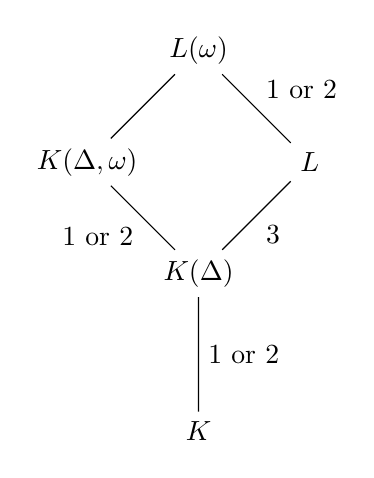
\begin{tikzpicture}[node distance=2cm]
        \node (Lw)                          {$L(\omega)$};
        \node (Kdw) [below left of=Lw]      {$K(\Delta, \omega)$};
        \node (Kd)  [below right of=Kdw]    {$K(\Delta)$};
        \node (L)   [below right of=Lw]     {$L$};
        \node (K)   [below of=Kd]           {$K$};

        \draw (K) -- (Kd)  node[midway,anchor=west]{1 or 2}
                  -- (L)   node[midway,anchor=north west]{3}
                  -- (Lw)  node[midway,anchor=south west]{1 or 2}
                  -- (Kdw)
                  -- (Kd)  node[midway, anchor=north east]{1 or 2};
    \end{tikzpicture}
\end{center}
From the \nameref{thm:towerLaw}, $\abs{L(\omega):K(\Delta, \omega)} = 3$. Hence $\Gal(L(\omega)/K(\Delta, \omega)) \cong C_3$.
We can apply \cref{thm:4.11} to see that $L(\omega) = K(\Delta, \omega)(\beta)$, where $\beta$ is a root of an irreducible polynomial $t^3 - \lambda \in K(\delta, \omega)[t]$.
In fact, from the proof of \cref{thm:4.11} we see that $\beta = \alpha_1 + \omega \alpha_2 + \omega^2 \alpha_3$ where $\alpha_1, \alpha_2, \alpha_3$ roots of $f(t)$.

Now all the extensions $K \leq K(\Delta) \leq K(\Delta, \omega) \leq L(\omega)$ are \hyperlink{def:cycloExt}{cyclotomic} or \hyperlink{def:kummerExt}{Kummer}.
So $f(t)$ is soluble by radicals.

\subsubsection*{In practice}
Given an irreducible cubic
\begin{align*}
    f(t) &= t^3 + at^2 + bt + c \\
         &= (t-\alpha_1)(t-\alpha_2)(t-\alpha_3)
\end{align*}
we have $\alpha_1 + \alpha_2 + \alpha_3 = -a$.

Replace the $\alpha_i$s by $\alpha_i' = \alpha_i + \frac{a}{3}$ so that $\alpha_1' + \alpha_2' + \alpha_3' = 0$.
They are roots of a polynomial $t^3 + pt + q$ and $K(\alpha_1,\alpha_2,\alpha_3) = K(\alpha_1',\alpha_2',\alpha_3')$.
We have $\hyperlink{def:disc}{D(g)} = -4p^3 - 27q^2$.

Set $\beta = \alpha_1' + \omega\alpha_2' + \omega^2\alpha_3'$, $\gamma = \alpha_1' + \omega^2 \alpha_2' + \omega \alpha_3'$. Then
\begin{align*}
    \beta\gamma &= \alpha_1' + \alpha_2' + \alpha_3' + (\omega + \omega^2) (\alpha_1'\alpha_2'+\alpha_1'\alpha_3'+\alpha_2'\alpha_3') \\
                &= (\alpha_1'+\alpha_2'+\alpha_3')^2 - 3(\alpha_1'\alpha_2'+\alpha_1'\alpha_3'+\alpha_2'\alpha_3') \\
                &= -3p
\end{align*}
and so $\beta^3 \gamma^3 = -27p^3$.
\begin{align*}
    \beta^3 + \gamma^3 &= (\alpha_1 + \omega \alpha_2' + \omega^2 \alpha_3')^3 + (\alpha_1' + \omega^2 \alpha_2' + \omega \alpha_3')^3 + (\alpha_1'+\alpha_2'+\alpha_3')^3 \\
                       &= 3(\alpha_1'^3 + \alpha_2'^3+\alpha_3'^3) + 18\alpha_1'\alpha_2'\alpha_3' \\
                       &= -27q
\end{align*}
since $\alpha_i'^3 = -p\alpha_i' - q$ and so $\alpha_1'^3 + \alpha_2'^3 + \alpha_3'^3 = -3q$.

So $\beta^3$ and $\gamma^3$ are roots of a quadratic $t^2 + 27qt - 27p^3$, hence they are
\begin{equation*}
    -\frac{27}{2}q \pm \frac{3\sqrt{-3}}{2} \sqrt{-27q^3 - 4p^3} = -\frac{27}{2} q \pm \frac{3 \sqrt{3}}{2} \sqrt{D}.
\end{equation*}
We can solve for $\beta^3$ and $\gamma^3$ in $K(\sqrt{-3}, \sqrt{D}) = K(\omega,\Delta)$.
We can get $\beta$ by adjoining a cube root of $\beta^3$, and then set $\gamma = \frac{-3p}{\beta}$.
Finally we solve in $L(\omega)$ for $\alpha_1', \alpha_2', \alpha_3'$ (remembering $\alpha_1'+\alpha_2'+\alpha_3'=0)$, using
\begin{equation*}
    \alpha_1' = \frac{1}{3}(\beta+\gamma), \quad \alpha_2' = \frac{1}{3}(\omega^2 \beta+\omega \gamma), \quad \alpha_3' = \frac{1}{3}(\omega\beta+\omega^2\gamma).
\end{equation*}

\subsection{Quartics}
As with the cubics by making a substitution of the form $\alpha_i' = \alpha_i + \frac{a}{4}$ we may assume the sum of the roots to be zero, and so the $t^3$ term is zero.

\begin{align*}
    f(t) &= t^4 + b t^2 + ct + d \quad \text{monic irreducible} \\
         &= (t - \alpha_1)(t-\alpha_2)(t-\alpha_3)(t-\alpha_4)
\end{align*}
Let $L = K(\alpha_1, \alpha_2, \alpha_3, \alpha_4)$ be the \hyperlink{def:splitting}{splitting field} for $f(t)$ over $K$ and set $M = L^{G \cap V_4}$.
The \nameref{thm:3.2} gives $\Gal(M/K) \cong \frac{G}{G \cap V_4}$.

\begin{center}
    \begin{tikzpicture}[node distance=2cm]
        \node (L) {$L$};
        \node (M) [below of=L] {$M=L^{G \cap V_4}$};
        \node (Kd) [below of=M] {$K(\Delta)$};
        \node (K) [below of =Kd] {$K$};
        \node [left of=M,align=center] {normal\\extension\\of $K$};

        \node (dummy) [right of=L] {};
        \node (e) [right of=dummy] {$\{e\}$};
        \node (Gv) [below of=e] {$G\cap V_4 \lhd G$};
        \node (Ga) [below of=Gv] {$G \cap A_4$};
        \node (G) [below of=Ga] {$G=\Gal(L/K)\leq S_4$};

        \draw (L) -- (M) -- (Kd) -- (K);
        \draw (e) -- (Gv) -- (Ga) -- (G);
    \end{tikzpicture}
\end{center}

Take $\theta: S_4 \to S_3$ with $\ker \theta = V_4$, so $S_4 / V_4 \cong S_3$.
Consider $\theta|_G : G \to S_3$, so $\ker \theta|_G = G \cap V_4$, and $\frac{G}{G \cap V_4} \cong \operatorname{im} \theta|_G \leq S_3$.

We therefore go looking for a cubic for which $M$ is the splitting field, called the resolvent cubic.

Set $x= \alpha_1 + \alpha_2$, $\gamma = \alpha_1 + \alpha_3$, $z = \alpha_1 + \alpha_4$ and so
\begin{align*}
    \alpha_1 = \frac{1}{2}(x+y+z),
    \alpha_2=\frac{1}{2}(x - y - z),
    \alpha_3=\frac{1}{2}(-x+y-z),
    \alpha_4=\frac{1}{2}(-x-y+z).
\end{align*}
Thus $K(\alpha_1, \alpha_2, \alpha_3, \alpha_4)=K(x,y,z)$.
\begin{align*}
    x^2=(\alpha_1+\alpha_2)^2&=-(\alpha_1+\alpha_2)(\alpha_3+\alpha_4)\\
    y^2=(\alpha_1+\alpha_3)^2&=-(\alpha_1+\alpha_3)(\alpha_2+\alpha_4)\\
    z^2=(\alpha_1+\alpha_4)^2&=-(\alpha_1+\alpha_4)(\alpha_2+\alpha_3)
\end{align*}

These are distinct, e.g.\ if $y^2=z^2$ then $y=\pm z$ and so either $\alpha_3 = \alpha_4$ or $\alpha_1 = \alpha_2$.
The $x^2,y^2,z^2$ are permuted by $G$ and are fixed by $G \cap V_4$ by observation.
So $K(x^2, y^2, z^2) \leq M = L^{G \cap V_4}$.

\textbf{Claim}: We have equality $M=K(x^2, y^2, z^2)$.
Consider the \textbf{resolvent cubic} $g(t) = (t-x^2)(t-y^2)(t-z^2) \in K[t]$.
Note that its coefficients are fixed by $G$ and so lie in $K$.

% Lecture 19
Observe $D(f) = D(g)$, (check on example sheet).
So $K(\Delta) \leq K(x^2, y^2, z^2)$. Now observe that $\Gal(L/K(x^2, y^2, z^2)) = \Gal(K(x,y,z)/K(x^2,y^2,z^2))$.
\begin{equation*}
    K(x^2,y^2,z^2) \leq K(x,y^2,z^2)\leq K(x,y,z^2) \leq K(x,y,z)
\end{equation*}
where each extension is degree 1 or 2.
So $\abs{K(x,y,z):K(x^2,y^2,z^2)}$ divides 8.
So, the elements of $\Gal(L/K(x^2,y^2,z^2))$ have order dividing 8.
But $\Gal(L/K(x^2,y^2,z^2)) \leq G \cap A_4$, so $\Gal(L/K(x^2,y^2,z^2)) \leq G \cap V_4$.
By the \nameref{thm:3.2}, $M=K(x^2,y^2,z^2)$. \qed

Consider the coefficients of $g(t)$: $x^2,y^2,z^2$ are permuted by $G$ and so the coefficients of $g(t)$ are fixed by $G$ and therefore in $K$.
\begin{align*}
    x^2+y^2+z^2&=-2b,\\
    x^2y^2+x^2z^2+y^2z^2&=b^2-4d,\\
    xyz=-c, \quad x^2y^2z^2&=c^2,\\
    \text{So } g(t)&=t^3+2bt^2+(b^2-4d)t-c^2
\end{align*}

We know how to solve cubics and so we can solve for $x^2, y^2, z^2$. Then we can solve for $x,y,z$.
Then use the formulae from earlier to find $\alpha_1, \alpha_2,\alpha_3, \alpha_4$.
\begin{center}
    \begin{tikzpicture}[node distance=2cm]
        \node (L) {$L$};
        \node (M) [below of=L] {$M$};
        \node (Kd) [below of=M] {$K(\Delta)$};
        \node (K) [below of =Kd] {$K$};
        \node [left of=M,align=center] {normal\\extension\\of $K$};

        \node (dummy) [right of=L] {};
        \node (e) [right of=dummy] {$\{e\}$};
        \node (Gv) [below of=e] {$G\cap V_4 \lhd G$};
        \node (Ga) [below of=Gv] {$G \cap A_4$};
        \node (G) [below of=Ga] {$G=\Gal(L/K)\leq S_4$};

        \draw (L) -- (M) -- (Kd) node[midway,anchor=east]{1 or 3} -- (K);
        \draw (e) -- (Gv) -- (Ga) node[midway,anchor=east]{1 or 3} -- (G);
    \end{tikzpicture}
\end{center}

\begin{eg}
    For $f(t) = t^4 + 4t^2 + 2$, we have $g(t) = t^3 + 8t^2 + 8t$ reducible.
\end{eg}

\subsection{Solubility by radicals}
Now suppose we have a \hyperlink{def:galoisExt}{Galois extension} $K \leq L$ with
\begin{equation*}
    K = L_0 \leq L_1 \leq \dotsb \leq L_m = L
\end{equation*}
such that $L_i \leq L_{i+1}$ is either \hyperlink{def:cycloExt}{cyclotomic} or \hyperlink{def:kummerExt}{Kummer} extension.

Let $G = \hyperlink{def:galoisGroup}{\Gal}(L/K)$. There is a corresponding chain of subgroups of $G$
\begin{equation*}
    G = G_0 \geq G_1 \geq \dotsb \geq G_m = \{e\}
\end{equation*}
with $G_i = \Gal(L/L_i)$, $L_i = L^{G_i}$ from \cref{thm:3.2}.

However each extension $L_i \leq L_{i+1}$ is Galois and we know
\begin{equation*}
    G_{i+1} = \Gal(L/L_{i+1}) \lhd \Gal(L/L_i) = G_i
\end{equation*}
hence $G_i / G_{i+1} \cong \Gal(L_{i+1}/L_i)$, which is abelian if $L_i \leq L_{i+1}$ is \hyperlink{def:cycloExt}{cyclotomic} and cyclic if $L_i \leq L_{i+1}$ is \hyperlink{def:kummerExt}{Kummer}.

\begin{ndef}[Soluble group]\hypertarget{def:soluble}
    A group is \textbf{soluble} if there is a chain of subgroups
    \begin{equation*}
        \{e\} = G_m \lhd G_{m-1} \lhd \dotsb \lhd G_1 \lhd G_0 = G
    \end{equation*}
    with $G_i / G_{i+1}$ abelian.
\end{ndef}

\begin{eg}\leavevmode
    \begin{itemize}
        \item $S_3$ is \hyperlink{def:soluble}{soluble}: $\{e\} \lhd \langle (123) \rangle \lhd S_3$.
        \item $S_4$ is soluble: $\{e\} \lhd V_4 \lhd A_4 \lhd S_4$ and $A_4/V_4 \cong C_3$, $S_4 / A_4 \cong C_2$.
        \item $A_5$ is simple, and therefore any normal subgroup is $A_5$ and so any chain would have a non-abelian quotient. So, $A_5$ is not soluble.
    \end{itemize}
\end{eg}
\begin{nlemma}\label{lem:4.16}
    A finite group $G$ is \hyperlink{def:soluble}{soluble} if and only if we have
    \begin{equation*}
        \{e\} = G_m \lhd G_{m-1} \lhd \dotsb \lhd G_1 \lhd G_0 = G
    \end{equation*}
    with $G_i/G_{i+1}$ cyclic.
\end{nlemma}
\begin{proof}
    $(\Leftarrow)$ is immediate.
    $(\Rightarrow)$. We know about the structure of finite abelian groups.
    If $A$ abelian then there is a chain
    \begin{equation*}
        \{e\} = A_r \lhd A_{r-1} \lhd \dotsb \lhd A_0 = A
    \end{equation*}
    with $A_r / A_{r+1}$ cyclic.
    Thus if we have a chain with abelian factors $G_i/G_{i+1}$ we can refine it to have cyclic factors.
\end{proof}
\begin{ndef}[Derived subgroup]\hypertarget{def:derivedSub}
    The \textbf{derived subgroup} $G'$ of a group $G$ is the subgroup generated by all the commutators $g_1 g_2 g_1^{-1} g_2^{-1}$ for $g_1 g_2 \in G$.
\end{ndef}
\begin{nlemma}\label{lem:4.18}
    Let $K \lhd G$. Then $G/K$ abelian $\iff \hyperlink{def:derivedSub}{G'} \leq K$.
\end{nlemma}
\begin{proof}
    \begin{align*}
        G/K \text{ abelian} &\iff Kg_1 Kg_2 Kg_1^{-1} K g_2^{-1} = K \quad \forall g_1, g_2 \in G\\
                            &\iff g_1 g_2 g_1^{-1} g_2^{-1} \in K \\
                            &\iff G' \leq K. \qedhere
    \end{align*}\qedhere
\end{proof}
\begin{remark}\leavevmode
    \begin{enumerate}[label=(\arabic*)]
        \item Next term in Representation Theory, we will prove Burnside's theorem: If $|G|=p^a q^b$ for $p,q$ distinct primes then $G$ is \hyperlink{def:soluble}{soluble}.
        \item The Feit-Thompson theorem says that if $|G|$ is odd, then $G$ is \hyperlink{def:soluble}{soluble}.
        \item There's an analogue of Sylow's theorems due to Philip Hall.
            For all $|G| = mn$ with $m,n$ coprime there is a subgroup of order $m$ iff $G$ is \hyperlink{def:soluble}{soluble}.
    \end{enumerate}
\end{remark}
\begin{ndef}[Derived series]\hypertarget{def:derivedSer}
    The \textbf{derived series} $\{G^{(m)}\}$ of $G$ is defined inductively:
    \begin{align*}
        G^{(0)} &= G \\
        G^{(1)} &= \hyperlink{def:derivedSub}{G'} \\
        G^{(2)} &= (G')' \\
        G^{(j+1)} &= (G^{(j)})' \\
    \end{align*}
    Thus $G = G^{(0)} \rhd G^{(1)} \rhd G^{(2)} \rhd \dotsb$ with $G^{(j)}/G^{(j+1)}$ abelian.
\end{ndef}
\begin{nlemma}\label{lem:4.20}
    For $G$ finite, $G$ is \hyperlink{def:soluble}{soluble} $\iff \hyperlink{def:derivedSer}{G^{(m)}} = \{e\}$ for some $m$.
\end{nlemma}
\begin{proof}
    If $G^{(m)} = \{e\}$ then the derived series gives a chain in the definition of solubility.

    Conversely if there is such a chain
    \begin{equation*}
        G \rhd G_1 \rhd G_2 \rhd \dotsb \rhd G_m = \{e\}
    \end{equation*}
    with $G_i/G_{i+1}$ abelian then an easy induction shows that $G^{(j)} \leq G_j$ and so $G^{(m)} = \{e\}$.
\end{proof}
\begin{nlemma}\label{lem:4.21}\leavevmode
    \begin{enumerate}[label=(\roman*)]
        \item Let $H \leq G$, $G$ \hyperlink{def:soluble}{soluble}. Then $H$ soluble.
        \item Let $H \lhd G$, then $G$ soluble $\iff H$ and $G/H$ both soluble.
    \end{enumerate}
\end{nlemma}
\begin{proof}\leavevmode
    \begin{enumerate}[label=(\roman*)]
        \item $G$ soluble $\implies \hyperlink{def:derivedSer}{G^{(m)}} = \{e\}$ by \cref{lem:4.20}.
            But $H^{(m)} \leq G^{(m)}$ and so $H$ soluble by \cref{lem:4.20}.
        \item Let $H \lhd G$, then $G$ soluble $\implies H$ soluble by (i).
            $G$ soluble $\implies G^{(m)} = \{e\}$, say.
            Observe that
            \begin{equation*}\hyperlink{def:derivedSub}{\left(\frac{G}{H}\right)'} = \frac{G'H}{H} \leq \frac{G}{H}.\end{equation*}
            Similarly,
            \begin{equation*}
                (\frac{G}{H})^{(j)} = \frac{G^{(j)}H}{H} \leq \frac{G}{H}.
            \end{equation*}
            Thus $(G/H)^{(m)} = H/H$, a trivial subgroup of $G/H$ and so $G/H$ soluble.

            Now consider the converse. Suppose that $H$ and $G/H$ are soluble.
            $H^({r}) = \{e\}$ and $(G/H)^{(s)} = H/H$.
            But
            \begin{equation*}
                \left(\frac{G}{H}\right)^{(s)} = \frac{G^{(s)}H}{H}
            \end{equation*}
            so $G^{(s)}H = H$ thus $G^{(s)} \leq H$. Hence $G^{(r+s)} \leq H^{(r)} = \{e\}$.
            Thus $G$ is soluble by \cref{lem:4.20}.
    \end{enumerate}
\end{proof}
\begin{eg}
    $S_5$ is not \hyperlink{def:soluble}{soluble} since its subgroup $A_5$ is not soluble.
\end{eg}
\begin{nthm}\label{thm:4.22}
    Let $K$ be a field and $f(t) \in K[t]$.
    Assume $\chara K= 0$. Then $f(t)$ is \hyperlink{def:radicals}{soluble by radicals} over $K \iff \hyperlink{def:ggPoly}{\Gal f}$ over $K$ is \hyperlink{def:soluble}{soluble}.
\end{nthm}
\begin{remark}
    We don't need to restrict to $\chara K = 0$. What we need to do for a particular $f(t)$ is to avoid a finite number of bad characteristics (avoid characteristics $\leq \deg f(t)$).
\end{remark}
\begin{ncor}\label{cor:4.23}
    If $f(t)$ is a monic irreducible polynomial $\in K[t]$ with $\Gal(f) \cong A_5$ or $S_5$ then $f(t)$ is not \hyperlink{def:radicals}{soluble by radicals} (with $\chara K$ = 0).
\end{ncor}
\begin{eg}
    In \cref{eg:3.9}, we considered $f(t) = t^5 - 6t + 3 \in \mathbb{Q}[t]$. $\Gal(f)$ over $\mathbb{Q}$ is $S_5$, and so $f$ is not \hyperlink{def:radicals}{soluble by radicals}.
\end{eg}
\begin{nlemma}\label{lem:4.24}
    If $K \leq N$ is an \hyperlink{def:radicals}{extension by radicals} then $\exists N'$ with $N \leq N'$ with $K \leq N'$ is an extension by radicals, with $K \leq N'$ a \hyperlink{def:galoisExt}{Galois extension}.
\end{nlemma}
\begin{proof}[Proof of \cref{thm:4.22}]
    Suppose $f(t)$ is \hyperlink{def:radicals}{soluble by radicals}.
    Thus if $L$ is the \hyperlink{def:splitting}{splitting field} of $f(t)$ over $K$ then $L$ lies in an extension of $K$ by radicals
    \begin{equation*}
        K = L_0 \leq L_1 \leq \dotsb \leq L_m
    \end{equation*}
    with each $L_i \leq L_{i+1}$ \hyperlink{def:cycloExt}{cyclotomic} or \hyperlink{def:kummerExt}{Kummer}.

    With \cref{lem:4.24}, we may assume $L_m$ is \hyperlink{def:galoisExt}{Galois} over $K$.
    By \nameref{thm:3.2} there is a corresponding chain of subgroups of $\hyperlink{def:galoisGroup}{\Gal}(L_m/K)$.
    Our previous discussion at the beginning of this section (before \cref{lem:4.13}) we know that $\Gal(L_m/K)$ is soluble.

    But $F \leq L \leq L_m$ with $K \leq L$ Galois.
    By \nameref*{thm:3.2}, $\Gal(L/K) \cong \Gal(L_m/K)/\Gal(L_m/L)$.

    But quotients of soluble groups are soluble, so $\Gal(L/K)$ is soluble.
\end{proof}
\begin{proof}[Proof of \cref{lem:4.24}]
    We have $K = L_0 \leq L_1 \leq \dotsb \leq L_m$ with each $L_i \leq L_{i+1}$ \hyperlink{def:cycloExt}{cyclotomic} or \hyperlink{def:kummerExt}{Kummer},
    and we want to embed this into a \hyperlink{def:galoisExt}{Galois} extension of the same form.

    Assume $\chara K = 0$. By the primitive element theorem, $L_m = \hyperlink{def:genField}{K(\alpha_1)}$ for some $\alpha_1$.
    Let $g(t)$ be the \hyperlink{def:minimalPoly}{minimal polynomial} of $\alpha_1$ over $K$ with \hyperlink{def:splitting}{splitting field} $M$.
    Thus $M = K(\alpha_1,\alpha_2,\dotsc,\alpha_n)$ where $\alpha_1, \dotsc, \alpha_n$ are roots of $g(t)$.

    There are \hyperlink{def:homo}{$K$-homomorphisms}
    \begin{align*}
        \phi_i : M &\longrightarrow M \\
        \alpha_1 &\longmapsto \alpha_i
    \end{align*}
    extending the $K$-homs $K(\alpha_1) \to K(\alpha_i) \leq M$.

    The tower $K \leq \phi_i(K) \leq \phi_i(L_1) \leq \dotsb \leq \phi_i(L_m) = K(\alpha_i)$ with cyclotomic or Kummer extensions as before,
    Consider $L_m = K(\alpha_1) \leq \phi_2(L_1)(\alpha_1) \leq \phi_2(L_2)(\alpha_1) \leq \dotsb \leq \phi_2(L_m)(\alpha_1) = K(\alpha_1,\alpha_2)$.

    Consider the extension $\phi_2(L_j)(\alpha_1) \leq \phi_2(L_{j+1})(\alpha_1)$:
    \begin{enumerate}[label={}]
        \item \textbf{if $L_j \leq L_{j+1}$ is cyclotomic} then all the roots of unity adjoined are now in $L_m = K(\alpha_1)$ and so $\phi_2(L_j)(\alpha_1) = \phi_2(L_{j+1})(\alpha_1)$.
        \item \textbf{if $L_j \leq L_{j+1}$ is Kummer} then we obtain $L_{j+1}$ by adjoining roots of an element of $L_j$ and so we obtain $\phi_2(L_{j+1})$ by adjoining roots of an element in $\phi_2(L_j)$.
            Hence we get from $\phi_2(L_j)(\alpha_1)$ to $\phi_2(L_{j+1})(\alpha_1)$ by adjoining roots of an element of $\phi_2(L_j)$. So it's a Kummer extension.
    \end{enumerate}

    Now continue to get suitable chain $K(\alpha_1,\alpha_2) \leq \dotsb \leq K(\alpha_1, \alpha_2, \alpha_3)$.

    Thus we get a suitable chain from $K$ to $K(\alpha_1, \dotsc, \alpha_n) = M$.
    Observe that $K \leq M$ is Galois.
\end{proof}

\begin{proof}[Converse of \Cref{thm:4.22}]
    Suppose $G = \hyperlink{def:ggPoly}{\Gal(f)}$ over $K$ is \hyperlink{def:soluble}{soluble} (and $\chara K=0$).
    Let $L$ be the \hyperlink{def:splitting}{splitting field} of $f(t)$ over $K$ and so $|G| = |L:K| = n$.
    Set $m = n!$ and let $\xi$ be a \hyperlink{def:primRoot}{primitive root of unity} and consider $L(\xi)$.
    \begin{center}
        \begin{tikzpicture}[node distance=2cm]
            \node (v) at (0,0) {};
            \node (Lx) [above of=v] {$L(\xi)$};
            \node (Kx) [left of=v]  {$K(\xi)$};
            \node (L)  [right of=v] {$L$};
            \node (K)  [below of=v] {$K$};
            \draw (Lx) -- (Kx) node[midway,anchor=south east]{$\leq n$} -- (K) -- (L) node[midway,anchor=north west]{$n$} -- (Lx);
        \end{tikzpicture}
    \end{center}
    Our proof is similar to that used for cubics.
    Observe that $|L(\xi):K(\xi)| \leq n$. By the \nameref{thm:2.17} $L=K(\alpha)$ for some $\alpha$ with \hyperlink{def:minimalPoly}{minimal polynomial} $g(t)$ say of degree $n$.
    Then $L(\xi) = K(\xi)(\alpha)$ and the minimal polynomial of $\alpha$ over $K(\xi)$ divides $g(t)$ and so is of degree $\leq n$.

    Then $\Gal(L(\xi)/K)$ is \hyperlink{def:soluble}{soluble} since $\Gal(L(\xi)/L)$ is soluble and $\Gal(L/K) \cong \frac{\Gal(L(\xi)/K)}{\Gal(L(\xi)/L)}$ soluble by \nameref{thm:3.2} and \Cref{lem:4.21}.
    Then the subgroup $\Gal(L(\xi)/K(\xi)) \leq \Gal(L(\xi)/K)$ is soluble by \Cref{lem:4.21}.

    Thus there is a chain of subgroups
    \begin{equation*}
        \Gal(L(\xi)/K(\xi)) = G_0 \rhd G_1 \rhd \dotsb \rhd G_m = \{e\},
    \end{equation*}
    with $G_i/G_{i+1}$ cyclic (using \Cref{lem:4.16}).

    Now use the \nameref{thm:3.2} to get a corresponding chain of fields $K(\xi) \leq K_1 \leq \dotsb \leq K_m = L(\xi)$, with each $K_i \leq K_{i+1}$ \hyperlink{def:galoisExt}{Galois}, with \hyperlink{def:cyclic}{cyclic} Galois group.
    By \Cref{thm:4.11}, all these extensions are Kummer (not all the extensions are of degree $\leq n$ and so we have the appropriate roots of unity).
    Thus we've embedded $L$ in an \hyperlink{def:radicals}{extension of $K$ by radicals}.
\end{proof}
\begin{eg}\leavevmode
    \begin{enumerate}[label=(\arabic*)]
        \item Take $f(t)=t^4+4t^2+2$, irreducible over $\mathbb{Q}$ by \nameref{thm:1.16}, and it has roots $\pm \sqrt{-2\pm\sqrt{2}}$ (two conjugate pairs).
            Complex conjugation gives double transposition.
            The resolvent cubic is $g(t) = t^3 + 8t^2+8t$ which is reducible with roots $0, -4 \pm 2 \sqrt{2}$.

            We have $L = K(\sqrt{-4+2 \sqrt{2}}, \sqrt{-4 - 2 \sqrt{2}})$, and $M = K(-4 + 2 \sqrt{2}, -4-2 \sqrt{2}) = K(\sqrt{2})$.
            So $|L:K|=8$, and the Galois group is dihedral.
        \item $f(t) = t^4 + 2t + 2$ is irreducible over $\mathbb{Q}$ by \nameref*{thm:1.16}.
            Its discriminant is $101 \cdot 4^2$, not a square, and the resolvent cubic is $g(t) = t^3 - 8t - 4$, irreducible since it is $t^3 + 2t+1$ mod 5, irreducible.
            So there is a 3-cycle in the \hyperlink{def:ggPoly}{Galois group}.

            $\Gal(f)$ is a transitive subgroup of $S_4$ and not of $A_4$ containing a 3-cycle, so $\Gal(f)$ is $S_4$.
        \item $f(t) = t^5-t-1$ is irreducible over $\mathbb{Q}$ since it is irreducible mod 5, and so the Galois group contains a 5-cycle and is a transitive subgroup of $S_5$.
            Mod 2, it factorises as a product of an irreducible cubic and quadratic: $(t^3+t^2+1)(t^2+t+1)$. So $\Gal(\bar{f})$ is generated by an element of cycle type $3,2$, so $\Gal(f)$ contains an element of cycle type $3,2$, so $g^3$ is a transposition.
            A subgroup of $S_5$ containing a 5-cycle and a transposition must be $S_5$ itself. So $\Gal(f) = S_5$ over $\mathbb{Q}$.
    \end{enumerate}
\end{eg}

\clearpage
\section{Final Thoughts}
\subsection{Algebraic closure}
\begin{ndef}[Algebraically closed]\hypertarget{def:closed}
    A field $L$ is \textbf{algebraically closed} if any $f(t) \in L[t]$ \hyperlink{def:splitting}{splits} into a product of linear factors in $L[t]$.
\end{ndef}
\begin{remark}
    This is equivalent to saying that any $f(t) \in L[t]$ has a root in $L$, or that any algebraic extension of $L$ is $L$ itself.
\end{remark}
\begin{ndef}[Algebraic closure]\hypertarget{def:closure}
    An extension $K \leq L$ is an algebraic closure of $K$ if $K \leq L$ is \hyperlink{def:algebraic}{algebraic} and $L$ is \hyperlink{def:closed}{algebraically closed}.
\end{ndef}
\begin{nlemma}\label{lem:5.3}
    If $K \leq L$ is \hyperlink{def:algebraic}{algebraic} and every polynomial in $K[t]$ \hyperlink{def:splitting}{splits} completely over $L$, then $L$ is an \hyperlink{def:closure}{algebraic closure} of $K$.
\end{nlemma}
\begin{proof}
    We need to show $L$ is \hyperlink{def:closed}{algebraically closed}.
    Suppose $L \leq L(\alpha)$ is a \hyperlink{def:degreeOfFieldExt}{finite extension}, and $f_\alpha(t) = t^n + a_{n-1} t^{n-1} + \dotsb + a_0$ is the \hyperlink{def:minimalPoly}{minimal polynomial} of $\alpha$ over $L$.
    Let $M = K(a_0, a_1, \dotsc, a_{n-1})$.
    Then $M \leq M(\alpha)$ is a finite extension.
    But each $a_i$ is \hyperlink{def:algebraic}{algebraic} over $K$ and so $\hyperlink{def:degreeOfFieldExt}{|M:K|}<\infty$.
    Hence $|M(\alpha):K| < \infty$ by \nameref{thm:towerLaw} and so $\alpha$ is algebraic over $K$.
    The minimal polynomial over $K$ must split over $L$, and so $\alpha \in L$.
    Thus any algebraic extension of $L$ is $L$ itself.
\end{proof}
\begin{eg}
    $\mathbb{A} = \set{\alpha \in C | \alpha \text{ \hyperlink{def:algebraic}{algebraic} over } \mathbb{Q}}$
    It is a subfield of $\mathbb{C}$: If $\alpha,\beta$ are \hyperlink{def:algebraic}{algebraic} over $\mathbb{Q}$ then $\hyperlink{def:degreeOfFieldExt}{|\mathbb{Q}(\alpha,\beta):\mathbb{Q}|} < \infty$ so if $\gamma = \alpha+\beta,\alpha-\beta,\alpha\beta$ or $\alpha/\beta$ (if $\beta\neq0$) we get $\mathbb{Q}(\gamma) \leq \mathbb{Q}(\alpha,\beta)$ and so $|\mathbb{Q}(\gamma):\mathbb{Q}<\infty$.
    So $\gamma$ is algebraic over $\mathbb{Q}$ so $\gamma \in \mathbb{A}$. Therefore $\mathbb{A} = \overline{\mathbb{Q}}$ is an \hyperlink{def:closure}{algebraic closure} of $\mathbb{Q}$.
\end{eg}
If we want to prove existence and uniqueness of algebraic closures in general then we need to appeal to Zorn's Lemma.
This appears in Logic and Set Theory, and it's equivalent to the Axiom of Choice and to the Well Ordering Principle.
\begin{ndef}[Partial order]\hypertarget{def:poset}
    $(\mathcal{S},\leq)$ is a \textbf{partial order} on $\mathcal{S}$ if
    \begin{enumerate}[label=(\roman*)]
        \item $\forall x \in \mathcal{S}$ $x \leq x$
        \item $x \leq y$ and $y \leq z \implies x \leq z$.
        \item if $x\leq y$ and $y \leq x$ then $x=y$.
    \end{enumerate}
    $\mathcal{S}$ is \textbf{totally ordered} if for any $x,y \in S$ either $x \leq y$ or $y \leq x$.
    A \textbf{chain} is a partially ordered set $(\mathcal{S},\leq)$ that is a totally ordered subset.
\end{ndef}
\begin{nlemma}[Zorn's Lemma]\label{lem:zorn}
    Let $(\mathcal{S},\leq)$ be a non-empty \hyperlink{def:poset}{partially ordered} set.
    Suppose that any \hyperlink{def:poset}{chain} has an upper bound in $\mathcal{S}$.
    Then $\mathcal{S}$ has a maximal element.
\end{nlemma}
\begin{nlemma}\label{lem:5.6}
    Let $R$ be a ring. Then $R$ has a maximal ideal.
\end{nlemma}
\begin{proof}
    Let $\mathcal{S}$ be the set of proper ideals of $R$.
    This is is non-empty, since $(0)$ is proper.
    Partially order $\mathcal{S}$ by inclusion.
    Any ideal $I$ is proper $\Longleftrightarrow 1 \notin I$.
    Any chain of proper ideals has an upper bound in $\mathcal{S}$, namely the union of the chain.
    \nameref{lem:zorn} gives that $\mathcal{S}$ has a maximal element, i.e.\ a maximal ideal of $R$.
\end{proof}

\begin{nthm}[Existence of algebraic closures]\label{thm:5.7}
    For any field $K$ there is an \hyperlink{def:closure}{algebraic closure}.
\end{nthm}
\begin{proof}
    Let
    \begin{equation*}
        \mathcal{S} = \set{(f(t),j) | f(t) \text{ irreducible, monic in } K[t], 1 \leq j \leq \deg f}
    \end{equation*}
    For each pair $s = (f(t),j) \in \mathcal{S}$ we introduce an indeterminate $X_s = X_{f,j}$.
    Consider the polynomial ring $K[X_s: s \in \mathcal{S}]$ and set
    \begin{equation*}\tilde{f}(t) = f(t) - \prod_{j=1}^{\deg g} (t - X_{f,j}) \in K[X_s: s \in \mathcal{S}][t].\end{equation*}

    Let $I \lhd K[X_s : s \in \mathcal{S}]$ generated by all the coefficients of all the $\tilde{f}(t)$.
    Denote the coefficents of $\tilde{f}(t)$ by $a_{f,l}$ for $0 \leq l \leq \deg f$.

    Claim: $I \neq K[X_s : s \in \mathcal{S}]$.
    Proof: Suppose $1 \in I$ and aim for a contradiction.
    \begin{equation*}
        b_1 a_{f_1,l_1} + \dotsb + b_N a_{f_N,l_N} = 1 \quad \text{in } K[X_s : s \in \mathcal{S}]. \tag{$+$} \label{eq:plus}
    \end{equation*}
    Let $L$ be a \hyperlink{def:splitting}{splitting field} for $f_1(t) \dotsm f_N(t)$.

    For each $i$, $f_i$ splits over $L$. $f_i(t) = \prod_{j=1}^{\deg f_i} (t-a_{ij})$.
    Define a $K$-linear ring homomorphism, identity on $K$,
    \begin{equation*}
        \begin{tikzcd}[row sep=tiny]
            \theta: K[X_s : s \in \mathcal{S}] \rar & L \\
            X_{f_i,j} \rar[maps to] & \alpha_{ij} \\
            X_s \rar[maps to] & 0 & \text{otherwise}.
        \end{tikzcd}
    \end{equation*}
    This induces a map $K[X_s : s \in \mathcal{S}] \to L[t]$.
    Then
    \begin{align*}
        \theta(\tilde{f}_i(t)) &= \theta(f_i(t)) - \prod_{j=1}^{\deg f_i} \theta(t - X_{f_i,j}) \\
                               &= f_i(t) - \prod_{j=1}^{\deg f_i} (t - \alpha_{i,j}) = 0.
    \end{align*}
    But then $\theta(a_{f_i,j}) = 0$ since $a_{f_i,j}$ are the coefficients of $\tilde{f_i}(t)$.
    But applying $\theta$ to \eqref{eq:plus} we get $0=1$.

    Then $I$ is a proper ideal of $K[X_s : s \in \mathcal{S}]$. By \nameref{lem:zorn} there is a maximal ideal $P$ of $K[X_s : s \in \mathcal{S}]$ containing $I$.
    Set $L_1 = K[X_s : s \in \mathcal{S}]/P$, a field.
    Thus we have a field extension $K \leq L_1$.

    Claim: $L_1$ is an \hyperlink{def:closure}{algebraic} closure of $K$.
    First show $K \leq L_1$ is \hyperlink{def:algebraic}{algebraic}: $L_1$ is generated by the maps $x_{f,j}$ of the $X_{f,j}$.
    However $\tilde{f}(t)$ has coefficients in $I$ and so its image $L_1[t]$ is the zero polynomial.
    Thus in $L_1[t]$,
    \begin{equation*}
        f(t) = \prod (t - x_{f,j}) \label{eq:23star}\tag{$*$}
    \end{equation*}
    and so $f(x_{f,j}) = 0$. Thus the $x_{f,j}$ are algebraic.

    Any element of $L_1$ involves only finitely many of the $x_{i,j}$ and so is \hyperlink{def:algebraic}{algebraic} over $K$.
    Moreover from \eqref{eq:23star} any $f(t) \in K[t]$ splits completely over $L_1$.

    The result follows from \Cref{lem:5.3}.
\end{proof}
\begin{nthm}\label{thm:5.8}
    Suppose $\theta: K \to L$ is a ring homomorphism and $L$ is \hyperlink{def:closed}{algebraically closed}.
    Suppose $K \leq M$ is an \hyperlink{def:algebraic}{algebraic extension}.
    Then $\theta$ can be extended to a homomorphism $\theta: M \to L$ (i.e.\ $\phi|_K = \theta$).
\end{nthm}
\begin{proof}
    Let
    \begin{equation*}
        \xi = \set{(N, \phi) | K \leq N \leq M, \phi \text{ a homomorphism } N \to L \text{ extending } \theta}.
    \end{equation*}
    Partially order $\xi$ with $(N_1, \phi_1) \leq (N_2, \phi_2)$ if $N_1 \leq N_2$ and $\phi_2|_{N_2} = \phi_1$.
    $\xi$ is non-empty since $(K, \theta) \in \xi$.

    If there is a chain $(N_1, \phi_1) \leq \dotsb$
    then set $N = \bigcup N_\lambda$. This is a subfield of $M$, and we can define $\psi: N \to L$ as follows:
    if $\alpha \in N$ then $\alpha \in N_\lambda$ for some $\lambda$ and we set $\psi(\alpha) = \phi_\lambda(\alpha)$. This is well defined.

    Then $(N,\psi)$ is an upper bound for our chain $\xi$.

    \nameref{lem:zorn} applies and gives a maximal element of $\xi$, $(N, \phi)$.
    We now show $N=M$.
    Given $\alpha \in M$, it is \hyperlink{def:algebraic}{algebraic} over $K$, and hence over $N$.
    Let $f_\alpha(t)$ be its \hyperlink{def:minimalPoly}{minimal polynomial} over $N$.
    But $\phi f(t)$ is in $L[t]$ and so splits completely over $L$, since $L$ is \hyperlink{def:closed}{algebraically closed}.

    So $\phi f(t) = (t-\beta_1)\dotsm(t-\beta_r)$, say.
    Since $\phi f(B_\gamma) = 0$ then there is a map
    \begin{equation*}
        \begin{tikzcd}
            N(\alpha) \cong \frac{N[t]}{(f\alpha(t))} \rar & L \\
            \alpha \rar[maps to] & \beta_1 & \text{extending} \phi
        \end{tikzcd}
    \end{equation*}
    Maximality of $(N,\phi)$ implies that $N(\alpha) = N$. So $\alpha \in N$, so $N = M$.
\end{proof}
\begin{nthm}[Uniquness of algebraic closures]\label{thm:5.9}
    If $K \leq L_1$, $L \leq L_2$ are two \hyperlink{def:closure}{algebraic closures} of $K$ then there exists an isomorphism $\phi:L_1 \to L_2$.
\end{nthm}
\begin{proof}
    By \Cref{thm:5.8} there is a homomorphism $\phi:L_1 \to L_2$ extending the embedding of $K$ into $L_2$.
    Since $K \leq L_2$ is algebraic, so too is $\phi(L_1)$. But $L_1$ is \hyperlink{def:closed}{algebraically closed} and so $\phi(L_1)$ is algebraically closed.
    So $L_2 = \phi(L_1)$ and $\phi$ is an isomorphism.
\end{proof}

\subsection{Symmetric polynomials and invariant theory}
In the buildup of the \nameref{thm:3.2} we met \nameref{thm:3.3}:
Let $K \leq L$ and $H$ a finite group of $\hyperlink{def:autGroup}{\Aut_K}(L)$. Let $M = L^H$. Then $M \leq L$ is a \hyperlink{def:galoisExt}{Galois extension} and $H = \hyperlink{def:galoisGroup}{\Gal}(L/M)$.

\begin{eg}
    $L = K(X_1, \dotsc, X_n)$. Let $S_n$ permute the variables.
    These permutations induce \hyperlink{def:homo}{$K$-automorphisms} of $L$.
    By \nameref{thm:3.3}, if $M = L^{S_n} \leq L$ then it is \hyperlink{def:galoisExt}{Galois} and $\Gal(L/M) = S_n$.
    Thus $S_n$ is a Galois group of some field extension.

\end{eg}
We know that we can regard any finite group $G$ as a subgroup of some $S_n$, and so we see that any finite group is a Galois group of some field extension (using \nameref{thm:3.2}).
Let
\begin{align*}
    f(t) &= (t-X_1)(t-X_2)\dotsm (t-X_n) \in M[t] \\
         &= t^n - s_1 t^{n-1} + s_2 t^{n-2} + \dotsb + (-1)^n s_n.
\end{align*}
Thus $s_1 = X_1 + \dotsb + X_n$, $s_2 = \sum_{i < j} X_i X_j$, and $s_n = X_1 X_2 \dotsm X_n$.
\begin{ndef}[Elementary symmetric polynomials]\hypertarget{def:esp}
    These $s_i$ are the elementary symmetric polynomials.
\end{ndef}
\begin{nthm}\label{thm:5.11}
    The fixed field $M = L^{s_n} = K(s_1, \dotsc, s_n)$ and the $s_1, \dotsc, s_n$ are algebraically independent over $K$ (in $L$).
\end{nthm}
\begin{ndef}\hypertarget{def:indep}
    $\alpha_1, \dotsc, \alpha_n$ are \textbf{algebraically independent} over $K$ if the ring homomorphism $K[Y_1, \dotsc, Y_n] \to K[\alpha_1, \dotsc, \alpha_n] \leq L$ is an isomorphism where $K[Y_1, \dotsc, Y_n]$ is the polynomial ring in $Y_1, \dotsc, Y_n$.
\end{ndef}
\end{document}
